
\chapter{人工智能:展望}

\section{“差一点儿出现”的情景与虚拟情景}

我的一个朋友读过《对实》之后对我说:“我叔叔差一点儿就是美国总统了!”“真的?”我问。“敢情,”他答道,“他当时是$108$号鱼雷艇艇长。”(约翰·肯尼迪曾任$109$号鱼雷艇艇长。)

这就是《对实》的全部意义所在。在日常思维中,从我们面临的情况、我们拥有的想法、客观发生的事件之中,我们总会构造出一些精神上的“变奏曲”,让某些性质基本保持原样,而让另一些性质发生“滑动”,从而形成一些“虚拟的”——我叫它们“对实的”情景。哪些性质是我们允许滑动的?哪些是我们根本不会考虑让其滑动的?在某种较深的直觉层次上,哪些事件被感知成是与确实发生的事件紧密相关的?有哪些事情会被我们看作“差一点儿”发生,或者“本当”发生了,但它们事实上没有发生?当我们听人讲故事时,哪些可能的结局会自然而然地出现在我们的脑海里?为什么我们会觉得某些虚拟事件比其它一些“虚拟得少点”?归根结底,没发生的事件显然就是没发生。在这里不存在一个“未发生度”。对“差一点儿”出现的情况也是一样。有时某个人会伤心地说“它差一点儿就发生了”,而另一个时候他又会欣慰地说同一句话。但这种“差一点儿”是存在于思想中的,并非存在于外界事实里。

假设你驾车行驶在乡间公路上,迎面碰上一群蜜蜂。你不仅会及时注意到它们,而且整个情景会立即在脑海中产生一群“重放的镜头”。典型地,你会想“幸亏我没开车窗”——或不幸是其反面:“糟糕,车窗没关!”;还可能是“幸亏我没有骑自行车来!”;“我怎么没早来五秒钟呢?!”;另一些奇特但可能出现的想法是“如果这是一头牛,我就已经完蛋了!”;“我敢打赌,这些蜜蜂更愿意碰上一棵玫瑰。”;甚至还有更怪的念头:“这些蜜蜂要都是钞票就好!”;“幸亏这些蜜蜂不是水泥的!”;“倒霉,为什么蜜蜂是一群而不是一只呢?”;“我是我,而不是蜜蜂,这可是万幸!”哪些滑动是自然的?哪些不是?为什么?

在最近的一期《纽约客》杂志上,重新引用了《费城迎客报》中的一段话:\note{《纽约客》[\bn{New Yorker}],1977年9月9日出版,第107页。}

\begin{quote}
如果列奥纳多·达·芬奇是个女的,西斯廷教堂的天花板就不会被画上画了。
\end{quote}
《纽约客》评论道:

\begin{quote}
如果米开朗基罗是个连体双胞胎,那他完成这幅作品的时间就会减少一半。
\end{quote}
《纽约客》评论的要点不是说这种虚拟事件是“假的”,而是说抱这种念头——想改动一个特定人物的性别或数目——的人,未免有点不近情理。但具有讽刺意味的是,在同一期的一篇新书介绍中,下面的句子被毫不脸红地印出来了:

\begin{quote}
我想他\lnote{(非利鲁·弗兰克教授)}如果仍健在,一定会对这两本书表示非常欣赏的。\note{《纽约客》[\bn{New Yorker}],1977年9月9日出版,第140页。}
\end{quote}

可怜的弗兰克教授已不在人世了。一个人读到写于他去世之后的书,这无论如何是说不通的。那为什么没人对这个一本正经的说法进行嘲弄呢?在某种难以捉摸的意义下,这个例子中参数的改动不像前一个例子那样违反我们关于“可能性”的观念。有某种东西使得我们在这个例子里面比前一个例子更容易想象“其它一切都是照常不变的”。但这是为什么呢?我们要怎样对事件和人物进行分类,才能进一步知道哪些滑动是“有意义的”,哪些是“胡闹”呢?

不妨看看在下列表达之间进行滑动是多么自然吧:开始是一个没什么价值的陈述:“我不懂俄文”,而后是一个内容丰富一些的条件句“我要懂俄文就好了”,下一个是一个充满情感的主观想象:“我希望我已经懂俄文了”,最后是一个内容丰富的虚拟语句“如果我懂俄文,我就能读契科夫和莱蒙托夫的原文著作了。”如果心智在一个否定句中除了晦暗的障碍以外什么都看不到,那该是多么平淡乏味啊!一个活生生的心智总能发现通往充满了可能性的世界的窗口。

我相信,那种“差一点儿”发生的情况和潜意识中构造的主观想象,代表着洞察力的某种最丰富的潜在来源。靠这种洞察力,我们可以了解人类是怎样组织他们对世界的感知,并形成范畴的。这个观点的一个强有力的支持者是语言学家兼翻译家乔治·斯坦纳。他在他的著作《巴别塔之后》中写道:

\begin{quote}
假设、想象、条件、虚拟的句法和偶然的句法可能是人类语言的发生中心……\lnote{(它们)}不光是造成哲学和语言学中的一些麻烦,与它们有关的也不像有人感觉的那样仅限于将来时态。或许该把它们划归到更大的集合中,如“假设推测”或“可能的选择”。这些带“如果”的命题为人类的情感机制提供了基础……
\end{quote}

\begin{quote}
我们能够——同时也需要——对世界进行否定或“不定”,以便以别的方式来设想和表述……我们需要找一个词来描述语言的这种威力和这种意向:即谈论“其它情况”的能力……或许该叫它“替代”,以此来定义“不同于真实的情况”、虚拟命题、想象、愿望和遁词,我们用这些东西掌管着我们的头脑,并以它们为工具为我们自己构造了一个变动不居、充满幻想的生物环境和社会环境……
\end{quote}

最后,斯坦纳为虚拟事件唱了一首虚拟颂歌:

\begin{quote}
从我们已有的知识推测,假如没有这种幻想的、虚拟的、反决定论的语言工具,没有产生并存储在大脑皮质的“多余”部分中的语义能力,并以此来想象和表达那些在单调沉闷的生物性衰退和死亡之外的各种可能性,人类是几乎不可能生存至今的。\note{乔治·斯坦纳,《巴别塔之后》第215--227页。}
\end{quote}

这种“主观想象出的世界”的构造过程产生得如此随便、自然,以致于我们几乎没注意到自己在做些什么。我们从我们的幻想中选出一个世界,它在某种内在精神意义下接近于真实世界。我们把真实的东西和我们感觉“差不多”真实的东西相互比较。这样,我们就得到了某种难以捉摸的对实在的看法。对话中的树懒就是实在的变奏之中的一个滑稽可笑的例子——一种没有进入主观想象能力的智能动物(或至少它自己宣称没有这种能力——但你可能已经注意到,在它的话中充满了虚拟语句!)试想,如果我们没有这种滑出真实世界、进入“假如”世界之中的创造性能力,那我们的精神生活将是何等的贫乏啊!从人类思维过程研究的观点看,这种滑动是十分吸引人的,因为它大多发生于完全缺乏意识指引的情况下,这意味着对什么可以滑动、什么不能滑动的观察将为我们认识潜意识提供一个良好的窗口。

认识这种精神测度的性质的一种方式是“以其人之道,还治其人之身”。在对话中就是这样干的,即要求我们的“主观想象力”设想一个世界,其中和我们的预期相比恰好让主观想象力这个概念滑动了。在对话中,第一个虚拟的重放镜头——即回文斯没有出界——是一个非常自然的想象。事实上,这个想法来自一个人对我说过的一番平常而又凑巧的话,这个人在一场球赛中坐在我身旁。出于某种原因,他的话触动了我,使我思考是什么使得这种滑动如此自然,而另一些滑动——如改变比分——则不然。从这些想法中,我进一步考虑另一些或许是更难滑动的特征,例如天气(这反映在对话中)、比赛的种类(也在对话中)、甚至一些更离奇的变化(也在对话中)。我注意到,在某一情景中显得荒唐可笑的滑动在另一个情景中可能就很容易发生。例如,有时你会很自然地考虑如果球的形状变了会怎么样(如你在玩一个气没打足的篮球时),而另一些时候这个念头则绝不会进入你的脑海(如你在看一场橄榄球赛的电视转播时)。

\section{稳定性的分层}

当时我觉得(现在依然如此),某些事件(或环境)特征的可滑动性,取决于我们在一个什么样的嵌套环境集合中感知此事件(或环境)的发生。在这里,从数学中借用“常量”、“参量”和“变量”这几个词可能是有用的。数学家、物理学家和其他一些人在进行运算时常常会说“$c$是个常量,$p$是个参量,$v$是个变量”。他们的意思是这三者都是可变的(包括常量),但是,存在一种可变性的层次差别。在这些符号所表示的情景中,$c$构成一种全局条件,$p$构成一种全局性较弱的条件——它可以在$c$保持固定时变动,最后,$v$可以在$c$和$p$保持固定时变来变去。在$v$固定时设想让$c$和$p$变化,这是没有意义的,因为$c$和$p$构成了使$v$有意义的环境。例如,设想一个牙科医生,他有一排病人,而每个病人又都有一排牙齿。一个完全有意义的事是让病人保持固定而让他的牙齿变动——但让牙齿保持固定而让病人变动则是根本没有意义的。(虽然有时变动牙科医生还是挺有意义的……)

我们逐层构造了一个情景的心智表示。其中最低层构成了环境的最深刻的方面——有时这个层次低得根本无法变动。例如,我们世界的三维性是个非常根深蒂固的观念,我们中的大多数人都从没想过让它在头脑中滑动。它是一个恒定的常量。然后是这样一些层次:它们虽然不是永久固定的,但却构成了情景中暂时固定的方面。这些方面可以被称为背景假设——在心灵深处,你知道这些方面是可能改变的,但在大多数时候,你总是不假思索地把它们当作不变的方面。这些仍可以被称为“常量”。例如,当你去看橄榄球赛的时候,比赛规则就属于这种常量。再往后就是“参量”:你认为它们有更大的可变性,但暂时把它们当作常量。在一场橄榄球赛中,参量可能包括天气、参赛球队,如此等等。可能——或很可能——存在着多层参量。最后,我们到达了你关于情景的心智表示中最不稳定的那些方面——变量。这就是像回文斯的出界之类的东西,它们在脑海中很“散漫”,你不会介意让它们在短时间内偏离其真实值。

\section{框架和嵌套的环境}

“框架”这个词正流行于当今的人工智能研究中。它可以被定义为“环境的可计算的实例化”。这个词的普及应归功于马尔文·明斯基,他发表了不少关于框架的见解。在框架语言中,可以说情景的心智表示包含着彼此嵌套的框架。情景中的各种成分都有它自己的框架。我心里对嵌套的框架有个想象,用语言表达出来可能会是很有意思的。设想有若干个柜子,每一个柜子上可以装若干个抽屉(就像中药铺里的那种柜子)。一旦你选择了一个柜子,你就有了一个框架,而且在这个柜子上的装抽屉的洞中可以放进“子框架”。子框架本身又是一个这样的柜子。怎么可能把整个柜子插到另一个柜子中的一个抽屉槽里去呢?很容易:你可以把它压缩一下,使它变形,因为这毕竟是在想象中,不是真要这样干。在外面的这个框架中,可能有若干不同的抽屉槽需要填充,然后你可能要用抽屉(或子框架)来填充某些装在里面的柜子。这个过程可以递归地进行下去。

对一个柜子进行挤压和扭曲,使得它能被装进任何形状的槽中,这种生动的超现实主义想象或许是极其重要的,因为这说明当你迫使某概念进入一个环境时,它也被该环境所挤压和扭曲了。这样,如果你考虑的人是个橄榄球队员,那么此时你关于“人”的概念变成了什么样的呢?显然它已经被扭曲了,是被整个环境强加给你的。你已经把“人”这个框架插在框架“橄榄球赛”的一个槽里了。用框架进行知识表示的理论依赖于这样一个想法:世界是由半封闭的子系统构成的,其中每个子系统都能充当其它子系统的环境,并且在此过程中不会受到或造成太大的破坏。

关于框架的主要想法之一,就是让每个框架带有自己的一组预设值。与此相应的想象是给每个柜子的每个抽屉槽中都预先装上一个称为“缺席选择”的抽屉,但并不将其装紧。如果我对你说“画一段河岸”,你将会激发出一幅具有各种特征的视觉想象,而如果我再添加进一步的说明,例如“在干旱季节”、“长满垂柳”、或“惊涛拍岸”,则你可能会去掉那些特征中的大多数。槽中缺席值的存在保证了递归填充槽的过程具有终点。实际上你是在说“我自己将只填充外面的三层槽,其它的就用缺席项”。和缺席预设值并存,一个框架还包含关于其使用限制的知识,以及在超出其容许限度时转换到其它框架的启发式规则。

框架的嵌套结构使得你可以“拍摄特写镜头”——以足够近的距离观察对象的细节:你只需选择适当的子框架,然后是子框架的子框架,等等,一直推进到拥有你所需要的细节为止。这就像一本交通地图册,第一页是一张全国地图,然后是分省地图,如果你需要进一步的细节,甚至还会有城市的地图或某些大村镇的地图。你可以设想一本拥有任意详细程度的地图册,一直到一条街、一幢房子,一间屋子,等等。这就像使用一台配有放大倍数不同的透镜的电子显微镜一样,每片透镜都有它自己的用途。重要的是我们能利用所有这些不同的尺度,因为细节常常是不相干的,甚至只能起干扰作用。

由于不同的框架可以被任意地插进其它框架的槽中,这就有发生冲突或“碰撞”的潜在可能。那种用单一的、全局的观点对“常量”、“参量”、“变量”进行分层,以形成一个整齐划一的模式的想法,未免把问题过分简单化了。事实上,每个框架自己都有一个可变性的层次结构。正因为如此,分析我们如何感知一个复杂事件——如一场橄榄球赛,连同它的大量子框架、子子框架等等——才成为一种混乱得令人难以置信的工作。这一大堆框架是怎样相互作用的?如果某个框架说:“这个项是个常量”,而另一个框架说:“不,它是个变量!”,那这种冲突怎样才能得到解决呢?这是一些关于框架理论的更深更难的问题,对此我无法提供答案。关于框架到底是什么东西,以及如何在人工智能程序中实现它,至今仍没有一个完全一致的看法。我准备在下面几节中讨论其中的一些问题,并谈谈视觉模式识别中的一些谜题,我称之为“邦加德问题”。

\section{邦加德问题}

“邦加德问题”的一般形式是俄罗斯科学家莫·邦加德在其著作《模式识别》中给出的。一个典型的邦加德问题——在他的一百个问题中的第51号——见\fig{119}。

\begin{figure}
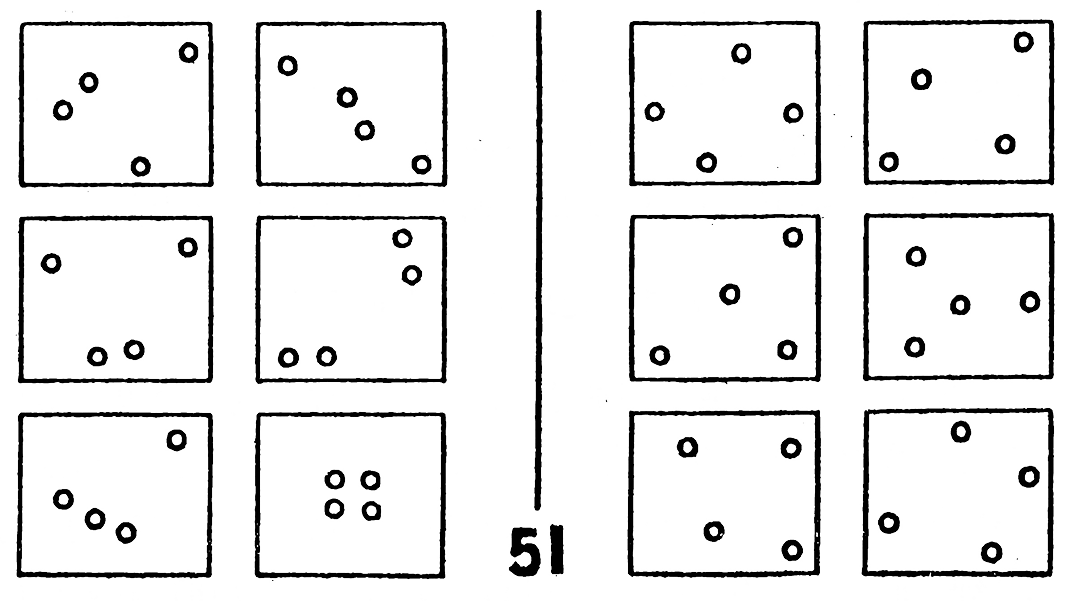
\includegraphics{img_119.png}
\caption[邦加德问题51号。]
  {邦加德问题51号。[摘自莫·邦加德,《模式识别》。]}
\end{figure}

这些有趣的问题是为模式识别者准备的,不管是人还是机器(也可以扔一个给外星人)。每个问题包括十二幅用方框围住的图像(以后简称为“框”):六个在左面,形成第I组,六个在右面,形成第II组。这些框可按下列方式编号:
\begin{center}
\begin{tabular}{ll!{\qquad}ll}
I-A&I-B&II-A&II-B\\
I-C&I-D&II-C&II-D\\
I-E&I-F&II-E&II-F
\end{tabular}
\end{center}
问题是“第I组和第II组中的框有何不同?”

一个求解邦加德问题的程序可能会包括若干阶段,原始数据通过它得以逐步转换成描述。初级阶段相对来说灵活性不大,而高级阶段逐渐变得更灵活一些。最终的阶段具有一种我称之为“尝试性”的性质,就是说一幅图像的表达方式总是带有尝试性的。只须出现微小的变化,用后面几个阶段提供的手段就能重新构造出一个高层描述来。下面要提出的想法本身也具有一定的尝试性。我将设法先传达总体想法,回避巨大的困难。然后我将回过头来设法解释那些微妙复杂之处。这样你在阅读时对于整个工作方式的认识也要经过某种修正。但这是体现在讨论的精神之中的。

\section{通过预处理选择微词汇表}

假设我们要解某个邦加德问题。题目被送到一台电视摄像机前,这样原始数据就被读进去了。然后对原始数据进行“预处理”,这就是说某些显著特征可以被检测出来。这些特征的“名字”构成了该问题的一个“微词汇表”,而它们是从一个通用的“显著特征词汇表”中抽取出来的。这个显著特征词汇表中的一些典型项是:

\begin{block}
线段、曲线、水平的、垂直的、黑的、白的、大的、小的、尖的、圆的……
\end{block}

在预处理的第二阶段,使用了某些关于“基本图形”的知识。如果发现了基本图形,它们的名字也要被包括进来。这样,可能会选出下列的项:

\begin{block}
三角形、圆形、矩形、凹入,凸出、直角、顶点、尖端、箭头……
\end{block}

在人脑中,这里差不多就是意识和潜意识的交汇点。以上的讨论主要是为了对此后发生的过程进行描述。

\section{高层描述}

至此,这幅图像已经根据某些已知的概念,在一定程度上被“理解”了,而且完成了一些检查工作。对于十二个框中的某一个或几个,已经作出了尝试性的描述。在这种描述中一般只使用下面这些简单的描述词:

\begin{block}
在上、在下、在左、在右、在里、在外、靠近、远离、平行、垂直、在一行中,分散的、间隔均匀的、间隔参差不一的、等等。
\end{block}
同时,还可能用到确定的或不确的数量描述词:

\begin{block}
$1$、$2$、$3$、$4$、$5$、……、许多、很少,等等。
\end{block}
以此可以构成较复杂的描述词,例如:

\begin{block}
在右方远处、不太靠近、几乎平行,等等。
\end{block}

\begin{figure}
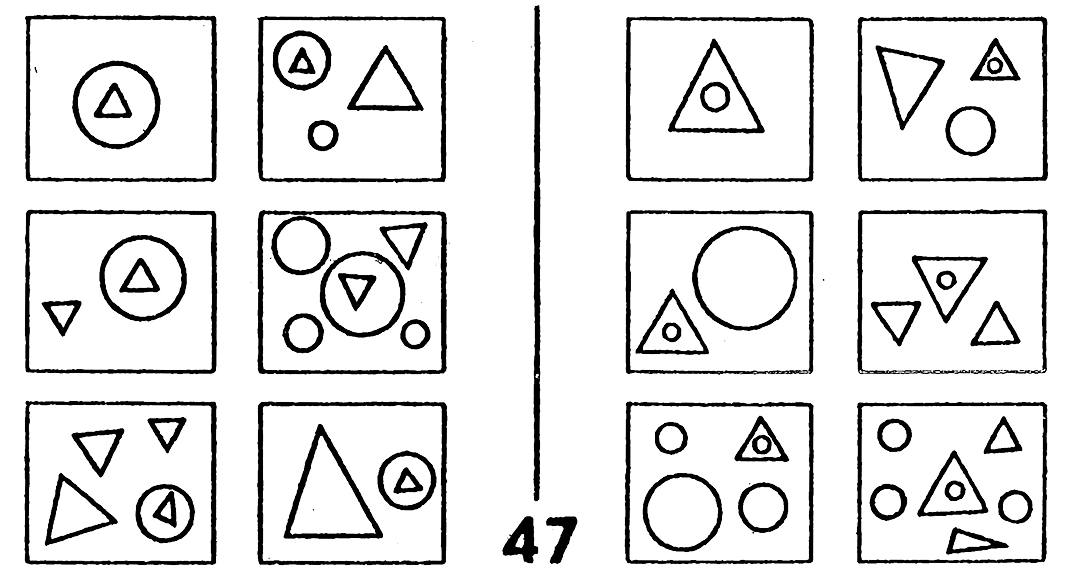
\includegraphics{img_120.png}
\caption[邦加德问题47号。]
  {邦加德问题47号。[摘自莫·邦加德,《模式识别》。]}
\end{figure}

这样,对一个典型框的内容——例如邦加德问题47号(\fig{120})中的I-F——可以有下列不同的描述:
\begin{center}
三个图形\\
或\\
三个白图形\\
或\\
右边有一个圆形\\
或\\
两个尖朝上的三角形\\
或\\
两个三角形和一个圆形\\
或\\
一个大图形和两个小图形\\
或\\
一个曲线图形和两个直边图形\\
或\\
一个里面和外面有同类图形的圆形
\end{center}

这些描述中的每一个都是通过一个“过滤器”来观察这个框的。脱离环境来看,其中每一个都可能是个有用的描述。但我们发现,在它们所处的特定的邦加德问题的环境中,它们全都是“错的”。换句话说,如果你知道邦加德问题47号中第I组和第II组的区别,然后给你一个上面那样的描述,作为对某个你未见到的图像的描述,那么这种信息将无法使你断定这个图像应该属于哪一组。在这个环境中,这个框的本质特征是它包括了:
\begin{block}
一个圆形包含一个三角形
\end{block}

注意,如果某个人听到了这一描述,他无法据此“重建”原始图形,但他能“识别”某个图形是否具有这种性质。这有点像音乐的风格:你可能会准确无误地辨别出莫扎特的作品,但同时又写不出一首能让别人以为是出于莫扎特之手的曲子来。

现在考虑一下邦加德问题91号(\fig{121})中的I-D框。在邦加德问题91号的环境中,一个繁琐然而是“正确”的描述是:
\begin{center}
一个带有三个矩形凹入的圆形。
\end{center}

\begin{figure}
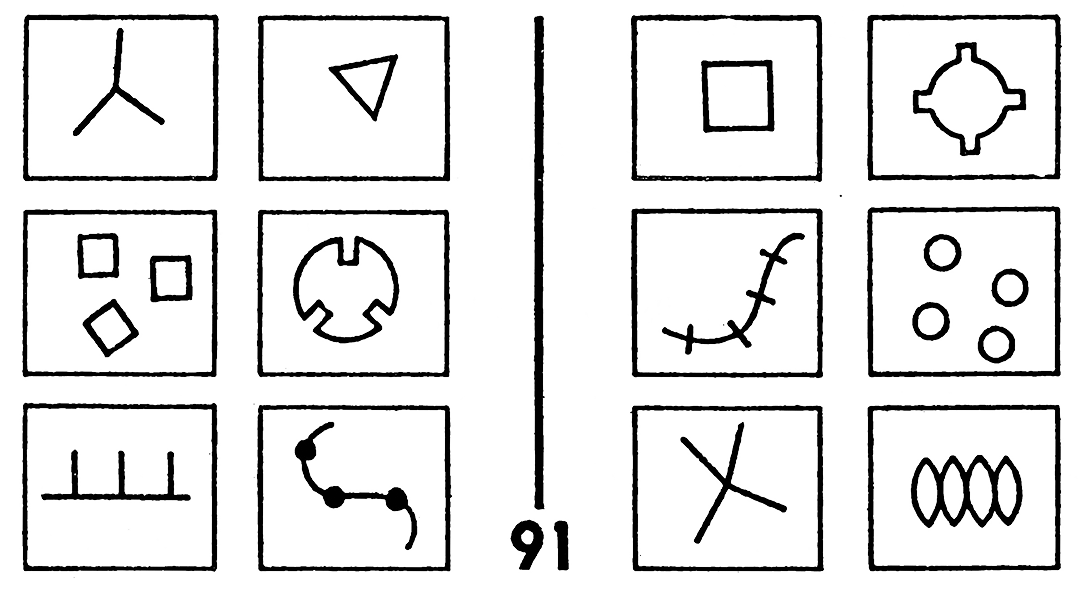
\includegraphics{img_121.png}
\caption[邦加德问题91号。]
  {邦加德问题91号。[摘自莫·邦加德,《模式识别》。]}
\end{figure}

请注意这种描述的复杂性,其中“带有”这个词起了某种否定作用,意思是那个“圆”实际上并不是个圆:它差一点就是个圆了,只是……进一步来说,凹入的也并非标准的矩形。在我们使用语言描述事物的方式之中,存在着许多“宽松”之处。显然,许多信息已经被扔掉了,甚至本应扔掉得更多些。想预先得知哪些该扔、哪些该留,这是很困难的。因此,为了得到一个适当的折中方案,必须采用恰当的方法。当然,如果不得不恢复已经丢掉的信息,那就需要求助于低层的描述了(即模块化程度较弱的描述),就好像人能够不断地观察该图形,以求重组关于它的想法一样。那么,关键就在于想出一些明确的规则来说明如何完成下列任务:
\begin{itemize}
\item 为每个框构造尝试性描述;
\item 把这些描述与两组中其它框的描述相比较;
\item 重新构造描述,用下列手段:
\begin{enumerate}[labelindent=0pt,label=(\roman*)]
  \item 添加信息,
  \item 去掉信息,或
  \item 从另一个角度看同样的信息;
\end{enumerate}
\end{itemize}
重复这一过程,直到发现能把两组图形区别开的东西为止。

\section{模板和同一性检测器}

尽最大可能使描述“在结构上彼此相似”,这可能会是个好的策略。它们所共同具有的结构将使它们之间的比较变得容易一些。在这种理论中有两个要素与该策略有关,其一是关于“描述模式”,或称“模板”的想法,其二是关于“同一性检测器”的想法。

先谈同一性检测器。它是出现在程序的各个层次上的“特派员”(事实上,不同的层次上可能会有不同种类的同一性检测器)。它不断地在个别的描述之中和不同的描述之间巡视,寻找重复出现的描述词或其它东西。一旦发现了某种同一性,就会触发各种重构操作,这既可能发生在单个描述水平上,也可能同时涉及多个描述。

现在来谈模板。在预处理完成后,首先要做的是设法构造一块模板,或者叫描述模式——一种适用于描述问题中所有框的“统一格式”。其基本想法是:描述常常可以通过某种自然的方式被分解成子描述,然后如果需要的话还可以把它们再变成子子描述。当你碰到属于预处理层次的基本概念时,这个分解过程就终止了。现在重要的是选择描述的分解方式,以反映所有框之间的共同点,否则将会引入一些多余而且无意义的“伪规律”。

\begin{figure}
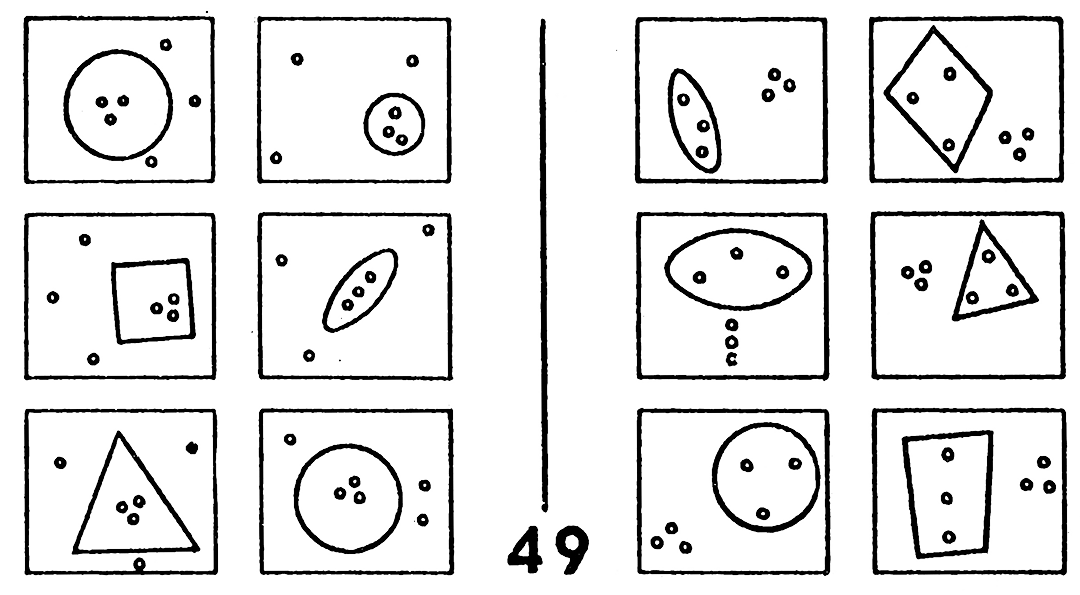
\includegraphics{img_122.png}
\caption[邦加德问题49号。]
  {邦加德问题49号。[摘自莫·邦加德,《模式识别》。]}
\end{figure}

模板是在什么样的信息的基础上被构造出来的呢?最好还是看一个例子。请看邦加德问题49号(\fig{122})。预处理得到的信息是每个框都包含若干个小圈和一个较大的封闭曲线。这个观察是很有价值的,应当被加到模板中去。这样关于模板的第一个设想可能是:
\begin{itemize}
\item 大封闭曲线:\blankline
\item 小圈:\blankline
\end{itemize}

这很简单:在描述模板中有两个明确的“槽”,需要用子描述来把它们填上。

\section{一个异层结构程序}

“封闭曲线”这个词触发了一件有趣的事情。这个程序中最重要的模块之一是一种语义网络——“概念网”,在这个网络中所有已知名词、形容词等等被相互联接起来了,而联接的方式就说明了它们的相互关系。例如,“封闭曲线”紧密地联接于“内部”和“外部”这两个词。概念网充满了关于词间关系的信息,例如谁和谁是相反的、谁和谁是相似的、谁和谁经常同时出现,如此等等。在\fig{123}中表示了一张概念网的一小部分,对此,我们不久就会加以解释。但让我们先来追寻在解决第49号问题时所发生的事情。“内部”和“外部”这两个词被激活了,因为它们在网络中与“封闭曲线”相邻。这就提示模板构造者:最好还能为该曲线的内部和外部分别设立槽。因此,根据“尝试性”的精神,模板被尝试着改组成下列形式:
\begin{itemize}
\item 大封闭曲线:\blankline
\item 内部的小圈:\blankline
\item 外部的小圈:\blankline
\end{itemize}

在找到子描述之后,“内部”和“外部”这两个词将调用有关过程去检查框中那些特定的区域。在邦加德问题49号中的I-A框内会发现下列情况:
\begin{itemize}
\item 大封闭曲线:\textit{圆形}
\item 内部的小圈:\textit{三个}
\item 外部的小圈:\textit{三个}
\end{itemize}
对同一个邦加德问题中的II-A框有下列描述:
\begin{itemize}
\item 大封闭曲线:\textit{雪茄形}
\item 内部的小圈:\textit{三个}
\item 外部的小圈:\textit{三个}
\end{itemize}

现在,一直和其它操作并行活动的同一性检测器发现,“三个”这个概念在所有和小圈有关的槽中同时出现,这就构成了着手进行第二次模板改组操作的一个强有力的理由。注意第一次是由概念网络建议的,而第二次是同一性检测器建议的。至此我们关于第49号问题的模板变成了:
\begin{itemize}
\item 大封闭曲线:\blankline
\item 内部的三个小圈:\blankline
\item 外部的三个小圈:\blankline
\end{itemize}

现在“三个”的普遍性已经提高了一层——也就是说进入了模板——因此也就值得去探索它在概念网中的邻居。其中一个是“三角形”,这就提示我们小圈组成的三角形可能是重要的。这实际上正好把我们带进了一条死胡同——但事先怎么可能知道呢?这是一条典型的、人所要探索的死胡同,因此如果我们的程序也能发现它,那反而是件好事了!对于II-E框来说,将会生成下列描述:
\begin{itemize}
\item 大封闭曲线:\textit{圆形}
\item 内部的三个小圈:\textit{等边三角形}
\item 外部的三个小圈:\textit{等边三角形}
\end{itemize}

当然这里已经丢掉了大量信息,包括这些三角形的大小、位置和方向,还有许多其它东西。但这恰恰是构造描述——不仅使用原始数据——的特点所在。我们在第十一章所讨论的“汇集”也体现了同样的想法。

\section{概念网络}

\begin{figure}
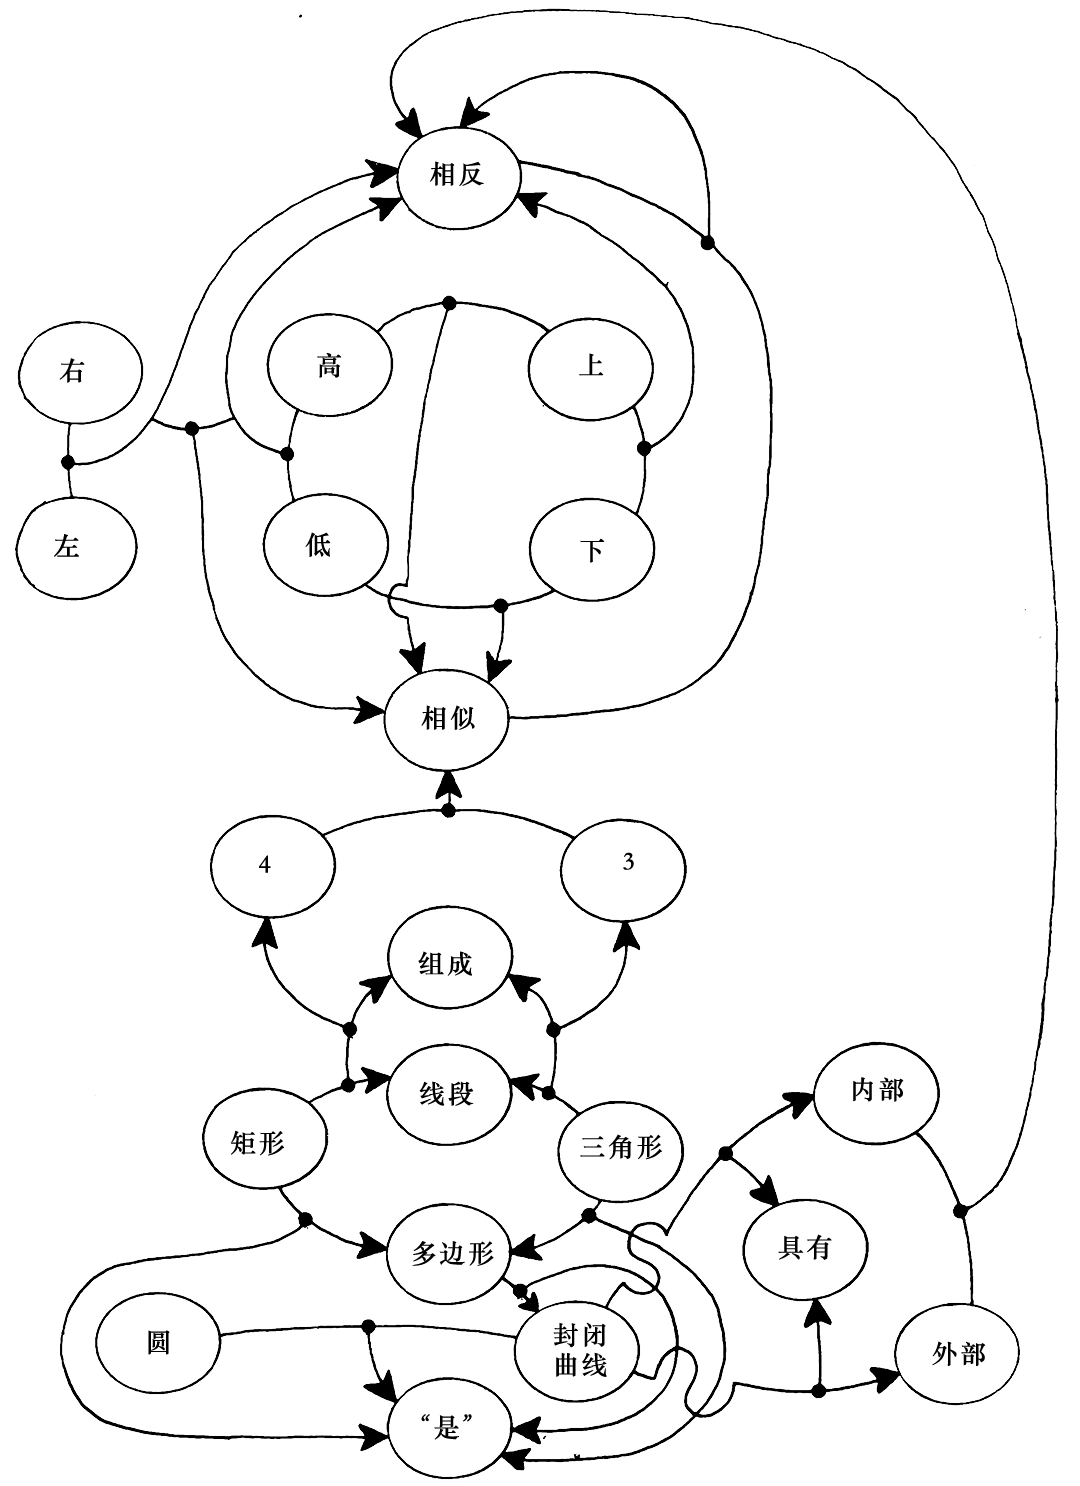
\includegraphics[height=.85\textheight]{img_123.png}
\caption[一个求解邦加德问题的程序的概念网络片段。]
  {一个求解邦加德问题的程序的概念网络片段。“结点”通过“连线”彼此相联,而连线又可能被联接。通过把连线看成动词,把它所联接的结点看成主语和宾语,你可以从图中抽取出一些句子来。}
\end{figure}

我们不必追寻第49号问题的整个解决过程,只需以此表明单个的描述、模板、同一性检测器和概念网络之间不断出现的反复的相互作用。我们现在应当更仔细地观察概念网络及其功能。\fig{123}中所示的一个简化了的网络片段表示了下列思想:
\begin{itemize}
\item “高”和“低”是相反的。
\item “上”和“下”是相反的。
\item “高”和“上”是相似的。
\item “低”和“下”是相似的。
\item “右”和“左”是相反的。
\item “左—右”差别相似于“高—低”差别。
\item “相反”和“相似”是相反的。
\end{itemize}

注意在网络中的一切东西——不论是结点还是连线——均可被描述。在此意义下,网络中任何东西都不比别的东西处于更高的层次。图中还显示了网络的另一部分,它表示了下列思想:
\begin{itemize}
\item 矩形是多边形。
\item 三角形是多边形。
\item 多边形是封闭曲线。
\item 三角形和矩形的差别在于一个有$3$条边,另一个有$4$条边。
\item $4$与$3$相似。
\item 圆是封闭曲线。
\item 封闭曲线具有内部和外部。
\item “内部”和“外部”相反。
\end{itemize}

概念网络必须非常大才行。它似乎只存储静态知识,或者叫描述性知识,而实际上并非如此。它的知识也可以说是过程性的,因为网络中的相邻性起到了引导者或“程序”的作用,可以告诉主程序如何深化它对框中图形的理解。

\begin{figure}
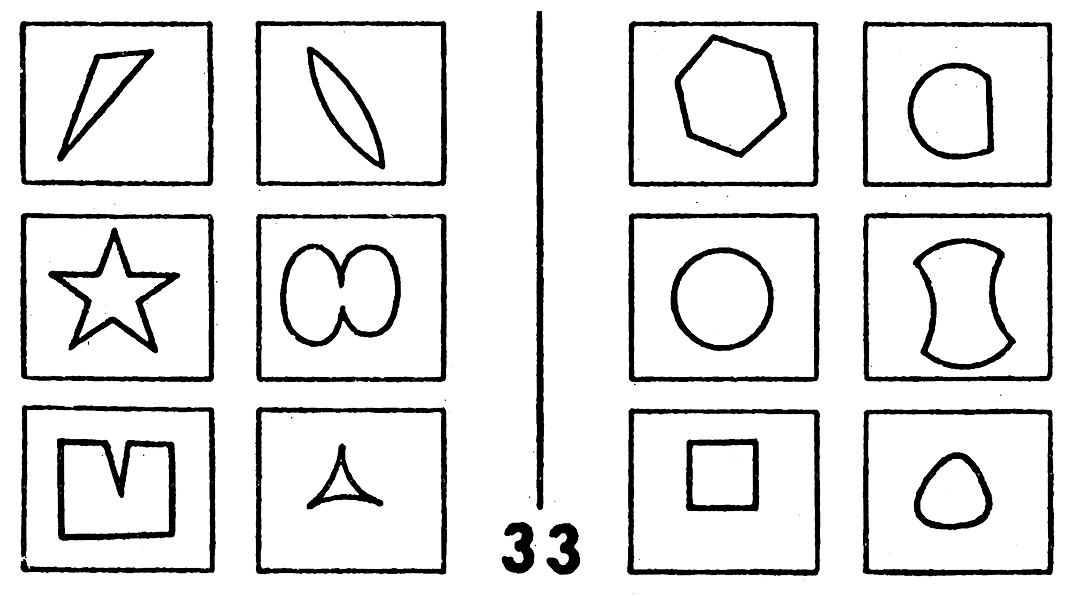
\includegraphics{img_124.png}
\caption[邦加德问题33号。]
  {邦加德问题33号。[摘自莫·邦加德,《模式识别》。]}
\end{figure}

例如,某些开始时的预感可能在后来被发现是错的,但其中包含着正确答案的萌芽。在邦加德问题33号(\fig{124})中,开始往往会产生的想法是:第I组的框都包含“有角的”图形,第II组的框都包含“平滑的”图形。但进一步考察就会发现这是错的。不过这种直感还是有价值的,我们可以把它进一步推向深入,在概念网络中考虑与“有角的”相邻的词。它与“锐角”这个概念相邻,而后者显然是第I组区别于第II组的特证。这样,概念网络的主要功能之一就是允许开始的错误想法被一点点修改,直至变成正确的。

\section{滑动和尝试性}

与在两个紧密相联的词间“滑动”这个概念有关的一个概念,就是把一个给定对象看作自另一个对象变化而来。我们已经提到过一个典型的例子——即“带有三个凹入的圆”,其中事实上根本没有圆形。我们必须具备在适当的时候使概念产生形变的能力。没有什么绝对不变的东西。在另一方面,也不能把事情弄得模棱两可,以致于完全丧失意义。关键在于要懂得该在什么时候以及用什么方式从一个概念滑向另一个概念。

邦加德问题85--87号(\fig{125})提供了一组很有趣的例子,其中的关键所在就是从一个描述滑向另一个描述的问题。邦加德问题85号很简单。让我们假设我们的程序在预处理阶段就能对“线段”进行标识。然后,对线段计数并找到邦加德问题85号中第I组和第II组的差别,这对它来说是比较容易的。现在来处理邦加德问题86号。它所用的一个一般性启发式规则是“设法找出最近行之有效的想法”。对最近用过的方法进行重复,这在现实世界中是非常普遍的,邦加德并不想把这种启发规则排除掉——事实上幸亏他强化了这一规则。这样我们就带着两个想法(“计数”和“线段”)着手分析第86号问题,而且这两个想法融成了一个:“对线段计数”。但实际上邦加德问题86号的关键是数“线列”而非“线段”,所谓“线列”是指一串首尾相连的线段(一条或多条)。程序发现这一点的可能方式之一是“线列”和“线段”二者均为已知,而且在概念网络中相邻。另一种方式是程序能“发明”“线列”这个概念——起码这是一个重要的前提。

\begin{figure}
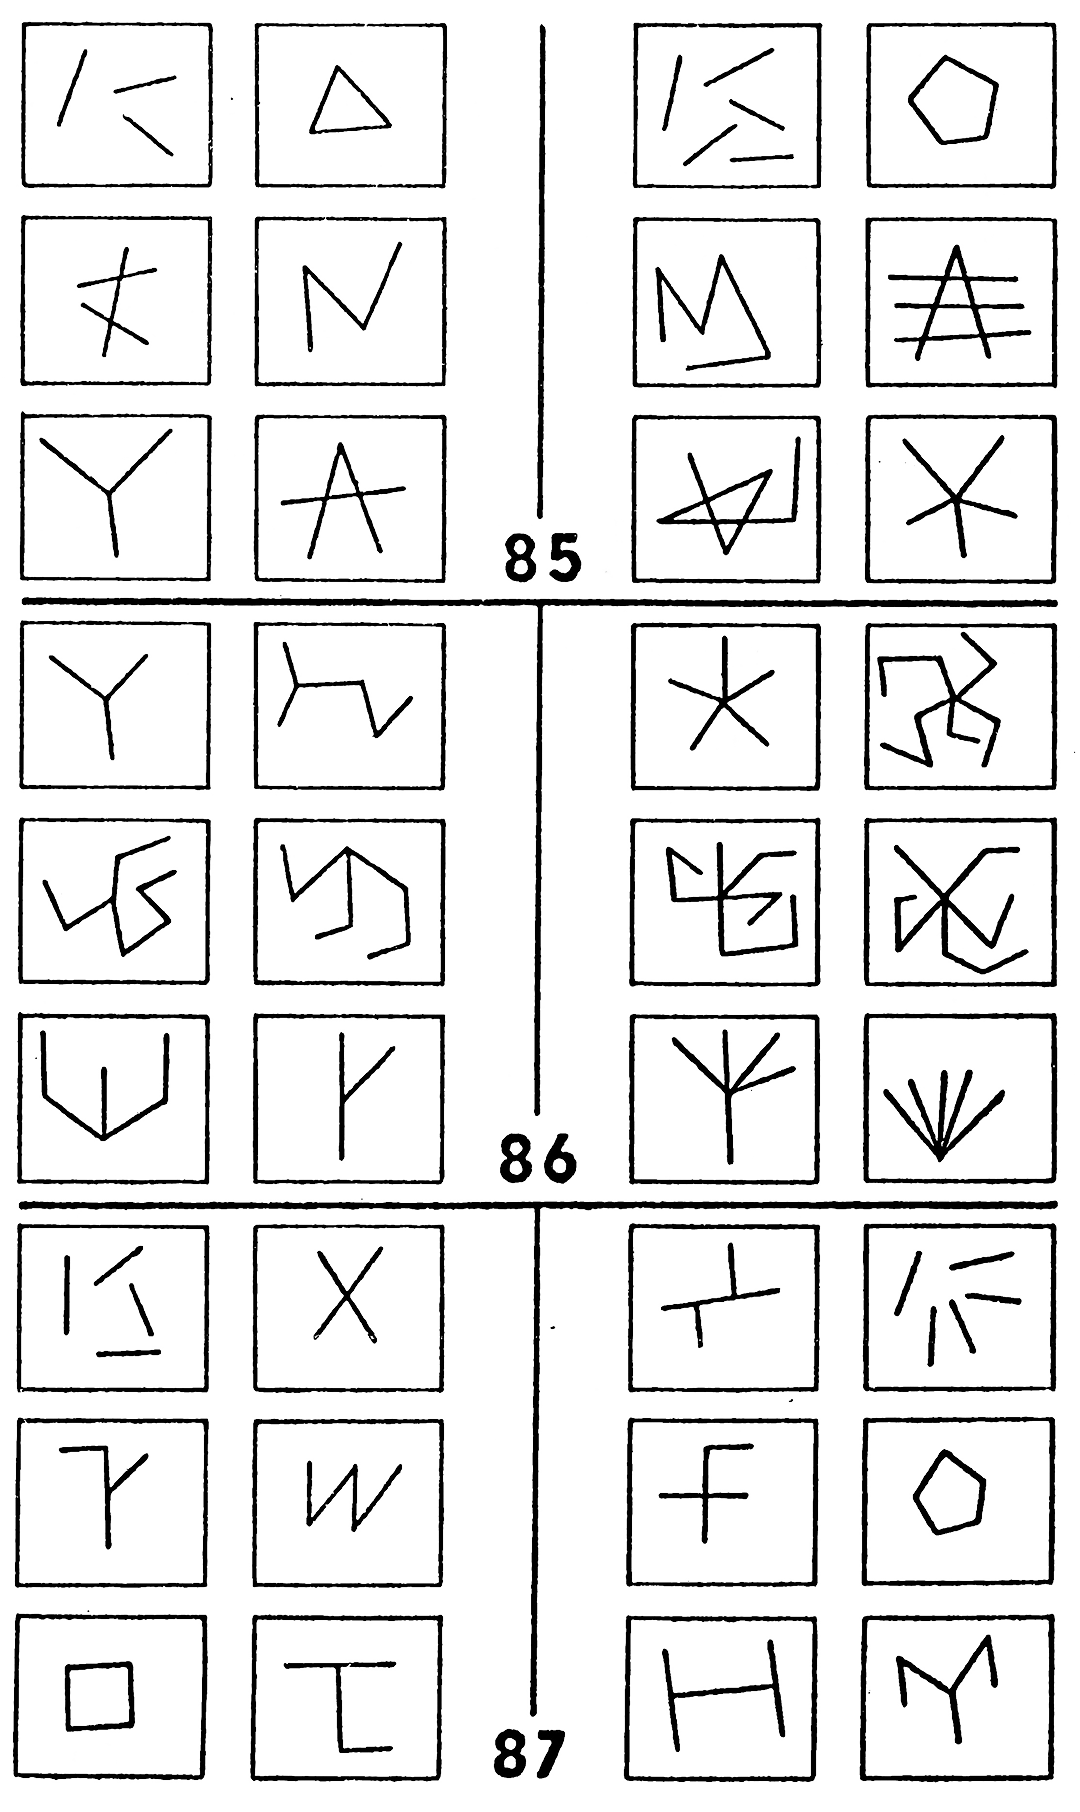
\includegraphics[height=.95\textheight]{img_125.png}
\caption[邦加德问题85--87号。]
  {邦加德问题85--87号。[摘自莫·邦加德,《模式识别》]。}
\end{figure}

下一个是邦加德问题87号,其中“线段”这个概念发挥了进一步的作用。什么时候一条线段会被当作三条线段?(见I-A框)程序应具有足够大的灵活性,才能在图形的给定部分的这种不同表示之间来往。一种明智的做法是把旧的表示方式存储起来,而不是把它们忘掉,否则可能还得把它们重建起来,因为谁也不能保证新的表示方式就一定比旧的好。这样,和每个旧表示方式一道,还应当存储一些喜欢它们或不喜欢它们的理由。(似乎开始复杂起来了,不是吗?)

\section{元描述}

至此我们将遇到识别过程的另一个至关重要的部分,它与抽象的层次和元描述有关。为此让我们再看一下邦加德问题91号(\fig{121})。在这里应当构造哪一种模板呢?情况实在太复杂,难以决定从何处下手。但这本身就是一条线索!这条线索说明,组与组之间的差别很可能存在于较高的抽象层次上,而不是存在于简单的几何描述之中。这个观察结果揭示程序应该构造“对描述的描述”——即“元描述”。或许在这个第二层上会出现某些共同特征,而且如果我们走运,就会发现足够多的共同点,以导致一个对元描述模板的精确刻划!因此我们在没有模板的情况下仍然往前走,为各种框构造描述。然后,一旦完成了这些描述,我们再描述它们。我们的元描述模板将有哪些种槽呢?或许包括这样一些:
\begin{itemize}
\item 所用的概念:\blankline
\item 重复出现的概念:\blankline
\item 槽名:\blankline
\item 所用的过滤器:\blankline
\end{itemize}
在元描述中可能还需要许多其它的槽,我们这里不过是举个例子而已。现在,假设我们已经对邦加德问题91号的I-E框作了描述。它的(无模板)描述可能会是这个样子:
\begin{itemize}
\item 水平线段
\item 立于该水平线段之上的垂直线段
\item 立于该水平线段之上的垂直线段
\item 立于该水平线段之上的垂直线段
\end{itemize}

当然许多信息已经被丢掉了:如三段垂直线段等长、等间隔的事实,等等。但上述描述是很有可能产生的。因此元描述可能会是这个样子:
\begin{itemize}
\item 所用的概念:垂直、水平、线段、立于
\item 描述中的重复:三次出现“立于该水平线段之上的垂直线段”
\item 槽名:\blankline
\item 所用的过滤器:\blankline
\end{itemize}

并非元描述中的所有槽都必须被填上。信息在这一层上可以像在“直接描述”层上一样被丢掉。

现在如果我们对第I组中的其它任何框构造描述,那我们每次都会在“描述中的重复”这个槽中填上“三次出现……”这个词组。同一性检测器会注意到这一点,并会选出“三次”作为第I组中的框在一个相当高的抽象层次上的一个显著特征。类似地,用元描述的方法,也会识别出第II组的标志是“四次”。

\section{灵活性是重要的}

现在你可能会提出异议,说在这种情况下求助于元描述方法就好像用高射炮打蚊子,因为三次和四次这种特征在低层次上会同样容易地被发现,只要我们在构造描述时稍微改变一下方式就行了。是的——但重要的是,沿不同的途径解决这些问题是完全可能的。在程序中可能存在着大量的灵活性,因此,即使程序一时“误入歧途”,这也是不足为怪的。在任何情况下,我都要阐明下列一般原理:一旦预处理器发现了大量差异,并因此使得模板难以构造,这本身就成了一条线索,说明这个问题牵扯到比预处理器所知道的东西抽象层次更高的概念。

\section{集聚与过滤}

现在让我们来看另一个问题:如何扔掉一些信息。这涉及到两个概念,我称它们为“集聚”和“过滤”。“集聚”是指构造这样一些描述:其焦点是框中图像的某一部分,而排除掉其它的部分。“过滤”是指构造这样一些描述:它以某种特定的方式来观察框的内容,而完全不顾其它方面。因此二者是互补的:集聚被用来处理客体(不严格地说,即名词),而过滤被用来处理观念(不严格地说,即形容词)。邦加德问题55号(\fig{126})就是有关集聚的一个例子。在这里,我们的注意力集聚于那个凹入和它旁边的小圆圈,而排除掉框中的其它成分。邦加德问题22号(\fig{127})提供了一个过滤的例子。在这里我们必须把除了图形大小之外的其它特性统统滤掉。而解决邦加德问题58号(\fig{128})的问题则需要把集聚和过滤结合起来。

\begin{figure}
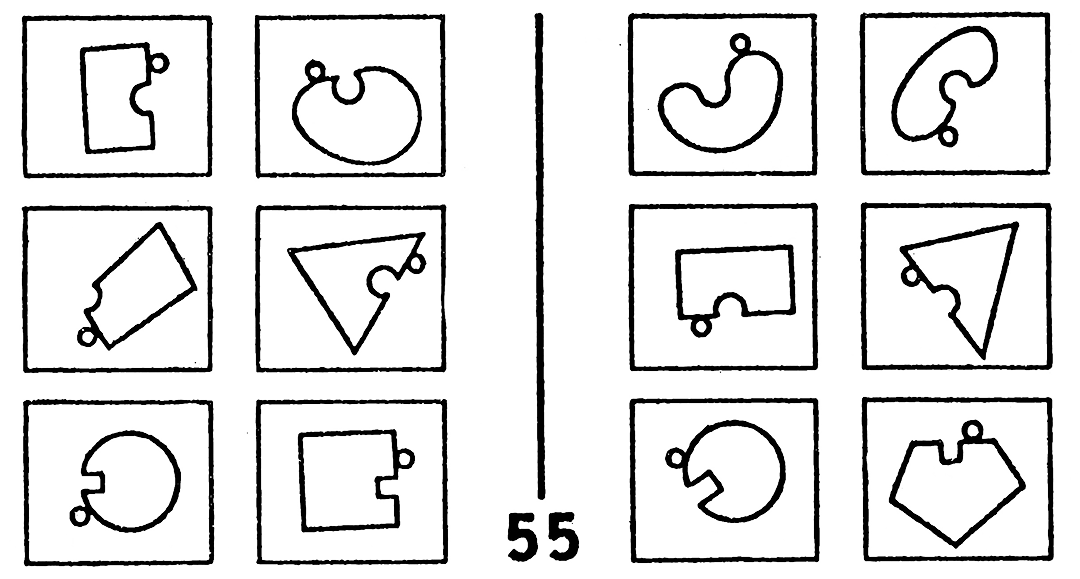
\includegraphics{img_126.png}
\caption[邦加德问题55号。]
  {邦加德问题55号。[摘自莫·邦加德,《模式识别》。]}
\end{figure}

\begin{figure}
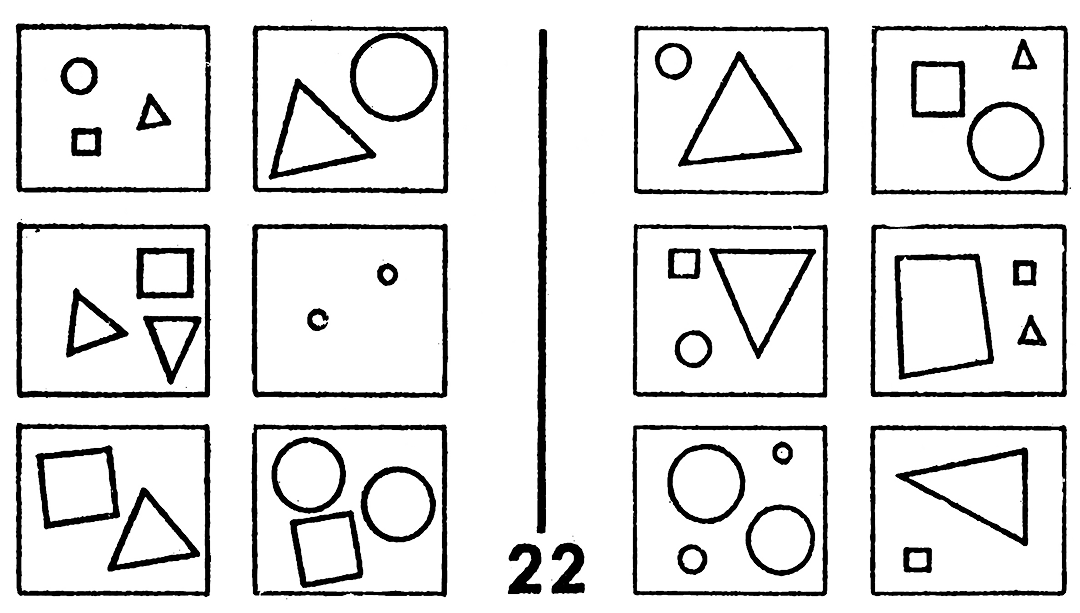
\includegraphics{img_127.png}
\caption[邦加德问题22号。]
  {邦加德问题22号。[摘自莫·邦加德,《模式识别》。]}
\end{figure}

\begin{figure}
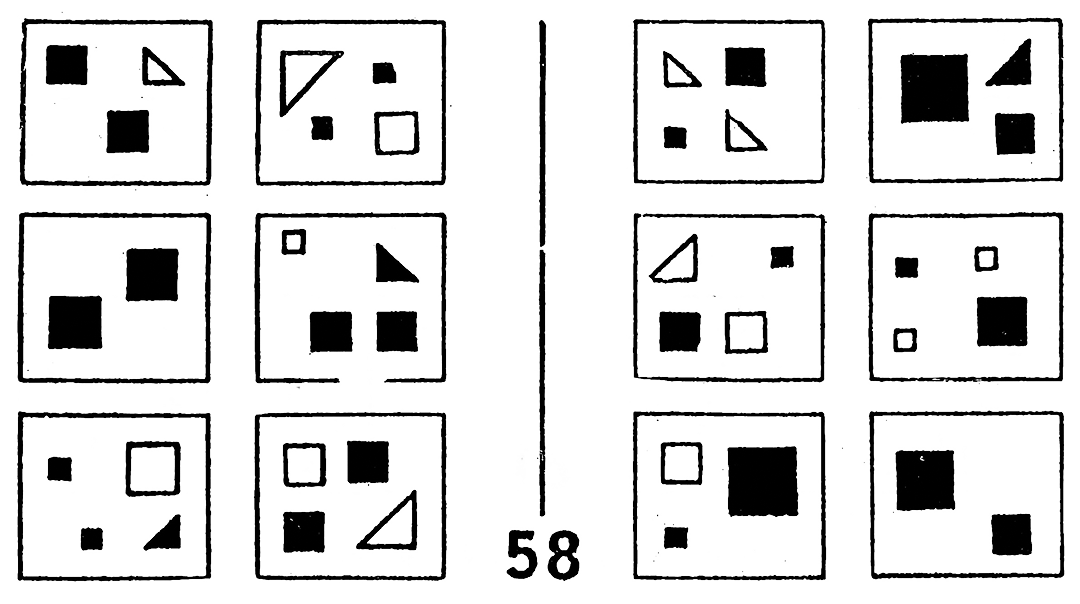
\includegraphics{img_128.png}
\caption[邦加德问题58号。]
  {邦加德问题58号。[摘自莫·邦加德,《模式识别》。]}
\end{figure}

为了找到集聚和过滤的方法,最重要的途径之一就是通过另一种“集聚”:即只检查一个特定的简单框——就是说其中的客体要尽可能少。一种非常有效的办法是把两组中最有代表性的框进行相互比较。但在得到描述之前,怎能说出哪些框是有代表性的呢?实际上检测代表性的一种方式就是寻找一个从预处理器那里得到的特征最少的框。这在一开始就可以确定,因为它不需要先准备好的模板。事实上,这可能是一种发现应构造在模板内的特征的有效方法。在邦加德问题61号(\fig{129})中,使用这种技术可以很快找到答案。

\begin{figure}
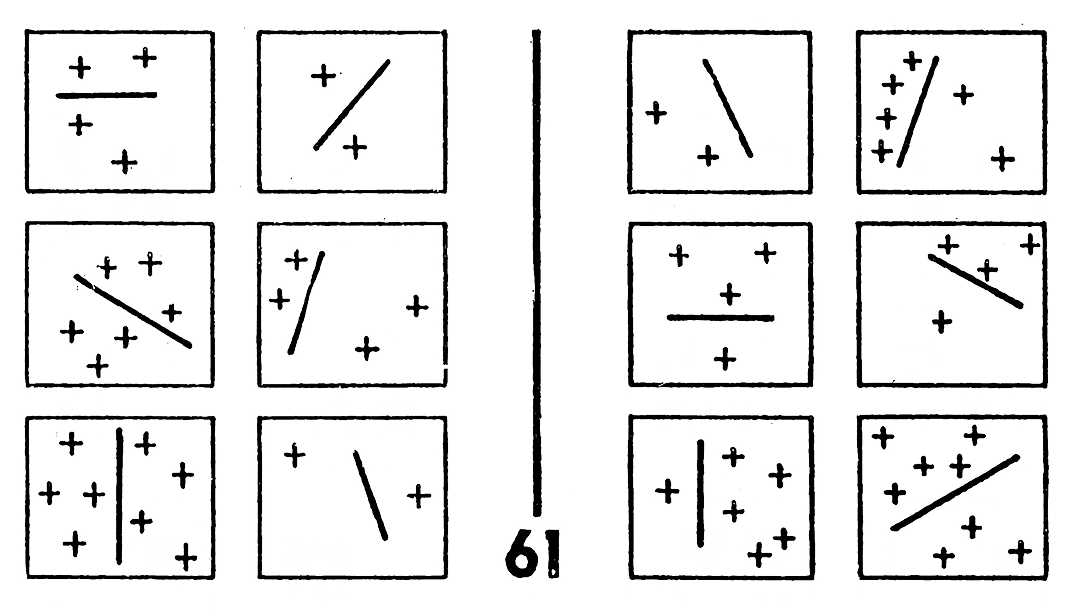
\includegraphics{img_129.png}
\caption[邦加德问题61号。]
  {邦加德问题61号。[摘自莫·邦加德,《模式识别》。]}
\end{figure}

\section{科学研究和邦加德问题的世界}

我们可以把邦加德问题构成的世界看成一个进行“科学研究”的小天地——也就是说,这种研究的目的是辨识该世界中的模式。在寻找模式的过程中,模板被装了又拆,拆了又装;槽的普遍性从一个层次转换到另一个层次;进行了集聚和过滤;如此等等。这里有复杂程度相差悬殊的各种发现活动。按照库恩的理论,某些被称为“范式转换”的罕见事件构成了“常规”科学与“观念革命”之间的分水岭。但这种观念似乎不适用于我们所讨论的问题,因为我们可以看到,在该系统中范式转换是随时随地都在发生的。描述的流动性使得范式转换可能以各种不同的规模发生。

当然,某些发现比另一些具有更大的“革命性”,因为它们的影响更为广泛。例如,有人可能会发现第70和71号问题(\fig{130})在一个足够抽象的层次上是“同一个问题”。关键是要看出二者都包含了二级嵌套和一级嵌套间的对比。这对邦加德问题来说是一个新的发现层次。甚至还有一个更高的层次,即把所有邦加德问题看成一个整体。如果有人从没见过这些问题,那把这些问题想出来本身就是个很好的问题。想出这些问题需要一种革命性的洞察力,但必须指出的是,使这种发现得以做出的思维机制与那种被用来解决一个具体的邦加德问题的思维机制并无不同。

\begin{figure}
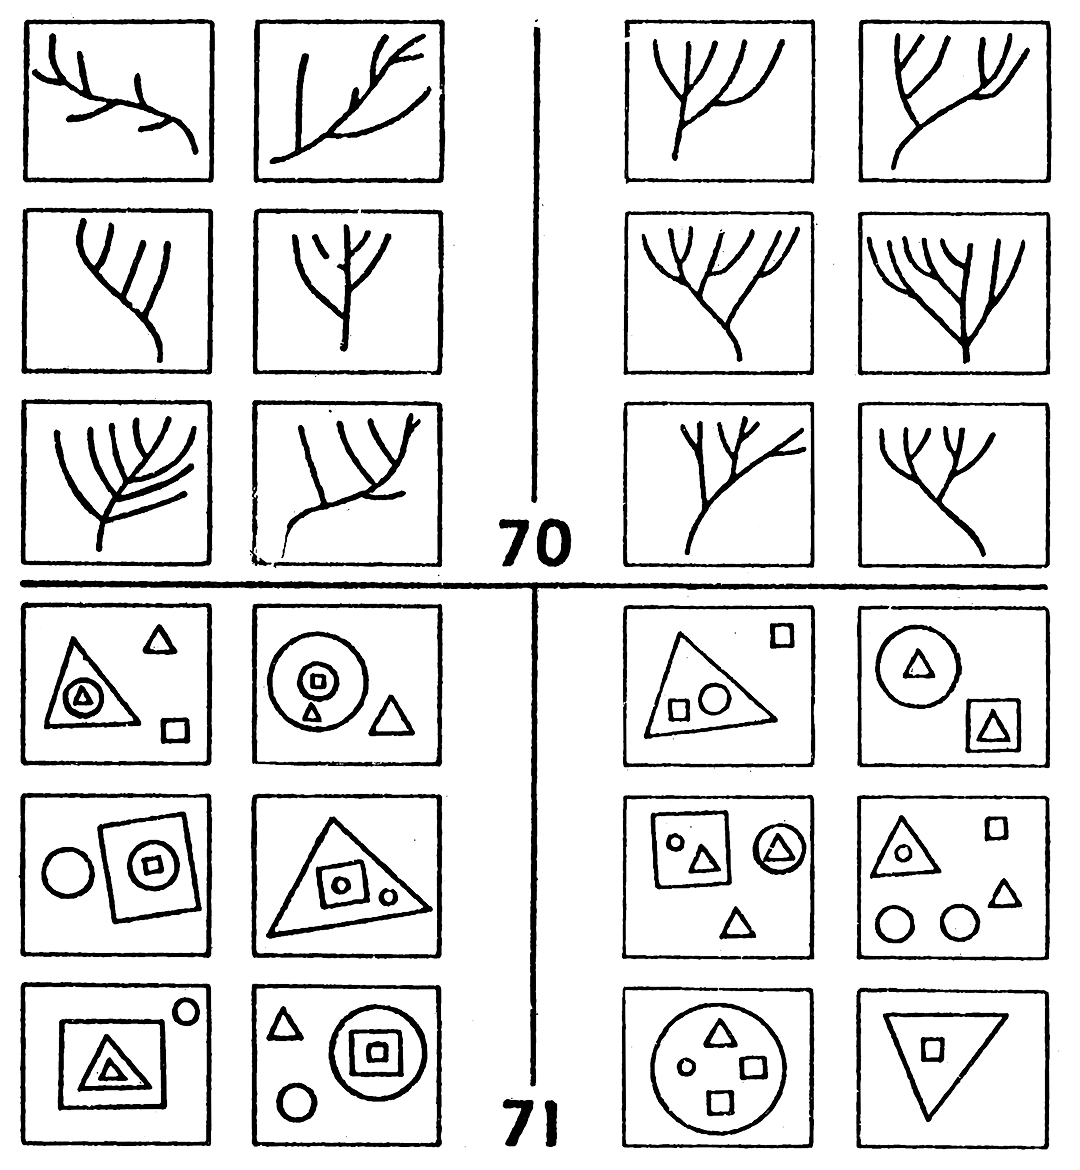
\includegraphics{img_130.png}
\caption[邦加德问题70--71号。]
  {邦加德问题70--71号。[摘自莫·邦加德,《模式识别》。]}
\end{figure}

根据同样的道理,起初的科学研究并不能被划分成“常规”阶段和“观念革命”阶段,而是充满了范式转换——它们之间只有大小之分和层次之别。INT和G图的递归图形(\fig{32}和\fig{34})为这种想法提供了一个几何模型:它们在每个层次上都具有不连续的跳跃,而不仅仅在最顶层是如此——只是层次越低跳跃幅度越小罢了。

\section{与其它类型思维的联系}

为了把这个完整的程序置于环境之中,让我们设想两种把它和认知的其它方面联系起来的方式。不仅它依赖于认知的其它方面,而且后者也反过来依赖于它。先让我说明一下它是怎样依赖于认知的其它方面的。要明白什么时候应忽略某些差别、尝试重新构造一个描述,以及回溯、转换层次等等,都是需要直觉的,而这种直觉可能只源于思维中的一般经验。因此,为程序的这些关键性的方面设计启发式规则可能是很困难的。有时,人关于世界中真实对象的经验对他描述或重新描述某些框的方式会产生微妙的影响。例如,谁知道某人对树木的熟悉能在多大程度上有助于他解决邦加德问题70号呢?我们无法断定对人来说与这些谜题有关的概念子网络是否能很容易地从整个网络中被分离出来。我们更倾向于相信一个人得之于观察和把握实在对象——如梳子、火车、线绳、木块、字母、橡胶带、等等——的直觉在解决这些谜题的过程中起着一种不可见的重要引导作用。

反过来,对真实世界情景的理解肯定极大地依赖于视觉表象和空间直觉,因此,如能以灵活有效的方式表示像邦加德问题中出现的那种模式,一定会对提高思维过程的一般效率有所贡献。

我觉得邦加德的问题都是精心设计出来的,它们具有一种普遍性,即每个问题的正确答案都是唯一的。当然有人会对此提出指责,说我们所谓的“正确”实际上是深刻地依赖于我们人类的,而其它星系中的生物可能会有完全不同的看法。虽然正反两种观点都缺乏具体证据,我还是确信邦加德问题取决于一种关于简单性的观念,而这种观念是不仅限于地球上的人类的。我在前面说过,熟悉梳子、火车、橡胶带等等地球所特有的物品或许是很重要的,但这并不排斥“我们关于简单性的观念具有普遍性”这种想法。原因是起决定作用的并不是这些个别物体,而是事实上它们一起确定了一个广阔的空间。很可能外星人和我们同样面对大量的人造或天然物体,而且也从中获得了大量经验。因此,我相信解邦加德问题所用的技巧位于离“纯粹”智能的核心很近的地方——如果这种所谓“纯粹”智能真的存在。因此,如果要研究发现模式或消息的“固有意义”所需的能力,那从这里着手是很合适的。遗憾的是我们只摘出了他的令人兴奋的题目中的一小部分。我希望读者们能从他的著作中(见参考书目)找到所有问题,并对它们有所了解。

有一些关于视觉模式识别的令人惊异的问题,我们人类似乎已将其完全“吸收”在潜意识之中了。这些问题包括:
\begin{itemize}
\item 识别面孔\lnote{(在年龄变化、表情变化、光线变化、距离变化、角度变化等之下的面孔不变性。)}
\item 在森林和山岭中识别足迹——这总以某种方式使我觉得是我们模式识别中最微妙的行为之一——动物也有这种本领
\item 流利地阅读以成百上千种不同的字型印出的文字材料
\end{itemize}

\section{传送消息的语言、框架和符号}

为了处理在模式识别和人工智能程序的其它应用中出现的复杂性,卡尔·海威特提出了所谓“演员”形式。(类似于艾伦·凯等人开发的“Smalltalk”语言)。根据这种方案,程序被写成一组相互作用的“演员”的集合,这些演员可以在彼此之间往返传送精心设计的“消息”。从某个角度看,这有点像一个由相互调用的过程所组成的异层结构集合。主要区别在于:过程间往返传送的参数通常数量很少,而演员之间相互交换的消息却可以任意长、任意复杂。

这种能够交换消息的演员在一定程度上成了有自主性的专职人员——事实上,甚至有点像自主的计算机,而消息就像其中的程序。每个演员都可以用自己特有的方式来解释任何给定的消息,这样,一条消息的意义将依赖于对它进行解释的演员。出现这种情况的原因是:演员都备有一段用来解释消息的程序,因此,有多少个演员就可能有多少个解释程序。当然,可能许多演员的解释程序是相同的,但这事实上将带来更大的好处,就好像在一个细胞中至关重要的是具有大量相同的核糖体,它们漂散在细胞质中,并都以一种共同的方式来解释消息——在这种情况下,消息是由RNA带来的。

一个有趣的问题是考虑一下如何把框架这个概念和演员这个概念结合起来。让我们把那种能生成和解释复杂消息的框架称为“符号”:
\[
\text{框架}+\text{演员}=\text{符号}
\]

我们现在已经是在讨论怎样实现在第十一章和第十二章中提到的那种难以捉摸的“活跃符号”了,因此在本章中,“符号”就是指那样的符号。顺便说一下,哪怕你不能马上看出这一综合是如何完成的,那也无须感到不安。虽然这一点显然是人工智能中最吸引人的发展方向之一,但也并非让人一目了然。进一步我们可以肯定,即便是对于这些概念的最佳综合,我们也将发现它的功能远弱于人脑中的实际符号。在这种意义下,把框架和演员的综合物称为“符号”未免为时过早,不过这提供了观察事物的一种最佳方式。

让我们转回到与传送消息有关的话题上来。每条消息是应当专门传向某个目标符号,还是应被扔到广阔的空间之中——像信使RNA被扔到细胞质中那样,去寻找接收它的核糖体?如果消息是有目标的,那每个符号就必须有一个地址,而传给它的消息就应当总是被送到那个地址。另一方面,也可能存在一个消息中心接收站,每条消息只须在那里老老实实等着,直到某个需要它的符号来把它取走。这对应于那种“存局待领”的邮件。或许最好的结论是允许两种类型的消息并存,同时满足不同类型的需要——专送邮件、快件、慢件等等。整个邮政系统为消息传送语言提供了丰富的思想,包括下列奇特的东西:备有回信地址和邮票的信封(发消息的人想尽快得到回信)、邮包(以某种很慢的方式传送非常长的消息)等等。如果你已经了解了邮政系统所包含的思想,电话系统会给你更多的灵感。

\section{酶与人工智能}

当然另一个消息传递——事实上,是一般信息加工——的丰富的思想源泉是细胞。细胞中的某些东西——特别是酶——很像演员。每种酶的活动场所都起着过滤器的作用,它只识别某种特殊的“底物”(即消息)。因此事实上每种酶都有一个“地址”。酶已经被“编了程序”(凭借其严整的结构)以完成那些对“消息”的操作,然后再将它释放出来。通过这种方式,一旦一条消息沿化学通道从一个酶被传送到另一个酶,就可以完成很多操作。我们已经描述过那种可能在细胞中发生的精致的反馈机制(通过抑制)。这些机制表明复杂的过程控制可以通过存在于细胞之中的各种消息传递来实现。

酶的最显著特性之一就是它们总是闲待在那里,等着被收到的底物所触发。然后,一旦这种底物来到,酶就会一下子跳起来投入行动,就像一棵捕蝇草一样。这种“一触即发”的程序已经被用在人工智能中,称为“精灵”。在这里重要的是下述想法:应当有许多种类不同的可触发子程序处于待触发状态。在细胞中,所有复杂的分子和细胞器都是通过一些简单步骤构成的。在这些新结构中,常常有些结构本身又是酶,而且它们又参与构造另外一些酶,如此下去。这种酶的递归“多级瀑布”能够对细胞的所作所为产生巨大影响。这种简单的逐步构造过程已经被引入人工智能之中,用于构造有用的子程序。例如,重复作用可以在我们头脑的硬件中形成新电路,因此经常重复的行为会变得被编码于意识水平之下。如果有一种类似的方法能对有效的代码片段进行综合,使它们能和在某个高层“意识”水平上学到的东西产生同样的操作序列,那将是极其有用的。酶的阶梯将为如何做到这一点提供一个模型(杰拉尔德·萨斯曼编写的“海客”程序对短小的子程序进行综合和调试的方式就有点像酶的阶梯)。

邦加德问题求解程序中的同一性检测器就可以用像酶那样的子程序来实现。同一性检测器可能会像酶那样带些随机性地东游西荡,不时在各处碰到小型数据结构。一旦在其两个“活性部位”上装入了同样的数据结构,该同一性检测器就会向程序的其它部分(演员)发出一条消息。只要程序还是顺序执行的,那么使用好几个同一性检测器的副本就没有太大意义,但在一个真正的并行计算机中,控制子程序的副本数,正是对一项操作被完成前的预期等待时间进行控制的一种方式。这就像在一个细胞中,控制了一种酶的副本数,也就控制了相应功能的完成速度。如果能综合生成新的同一性检测器,那就相当于在我们的头脑中使模式检测过程渗透到一个更低的层次。

\section{裂变与聚变}

“裂变”和“聚变”是两个有趣而且互补的想法,涉及到符号的相互作用。“裂变”是指一个新符号逐渐脱离它的母符号(即被用来为它做复制模板的那个符号)。“聚变”是指两个(或多个)原来互不相干的符号由于参与了某个“连带激活”,彼此频繁地往返传送消息,紧密地联系在一起,因而以后这个复合体可以被作为一个符号来访问。裂变或多或少是一个不可避免的过程,因为一旦一个新符号从老符号上被“剥下来”,它就变成自主的,而且在它自己的内部结构中反映出它与外部世界的相互作用,因此开始时的一个完全的复制品不久就会变成不完全的,而且此后慢慢会变得越来越不像那个它从其上被“剥下来”的符号。聚变是一个更为复杂的过程。什么时候两个概念才真的变成了一个?是否存在着某个发生聚变的确切时刻?

“连带激活”这个概念打开了一个装满了问题的潘多拉之匣。当我们提到某种“东西”时,我们是否想到了“东方”和“西方”?英文里的“chairman”[主席]到底与“chair”[椅子]和“man”[男人]有多少关系?(有人至今还在指责这种词充满了大男子主义)。一个德国人在说“手套”[Handschuhe]时是否真的想到了“穿在手上的鞋”(该词的字面意义)?到底这些部分在多大程度上与整体产生共鸣,恐怕是因人而异、因地而异的。

与符号的“聚变”这个概念有关的实际难题是:很难设想出一个通用的算法,能从相互碰撞的符号中构造出有意义的新符号来。这就像两条DNA碰到了一起。你怎样才能从它们中各取出一部分,把它们拼成一条有意义并且能活下去的新DNA,而且使它构成同一物种的一个个体——或一个新物种——的遗传编码?一次DNA片段的随机组合就构成了某种能存活的东西的遗传密码,这种可能性可以说是微乎其微——就像两本书中的词重新随机组合能得到另一本书的可能性一样。想让这种重组DNA在除最低层外的任何层次上仍有意义,这种可能性极其微小,其原因完全是由于在DNA中具有太多的意义层次。对“重组的符号”来说也是一样。

\section{《螃蟹卡农》的渐成过程}

我来把我写的对话《螃蟹卡农》当作一个典型事例。其中,有两个想法在我的头脑中发生碰撞,并以一种新方式联结起来了。这时,一种新语词结构突然活生生地出现在我的脑海中。当然我现在仍然可以分别考虑螃蟹卡农音乐和言语对话——它们仍能彼此独立地被激活,但《螃蟹卡农》对话所对应的合成符号也具有它自己所特有的激活方式。为了更详细地描述这个聚变或“符号重组”的概念,我想把我的《螃蟹卡农》的发展作为一个事例来研究。这当然是因为我对此比较熟悉,也还因为这个例子很有趣,而且很典型地说明了一个想法可以被推广到什么程度。我将列举其各个阶段,这些阶段是根据“成熟分裂”的各阶段来命名的,而“成熟分裂”是指那种伴随有“交换”——或称基因重组——发生的细胞分裂,这是进化中的多样性的来源。

\begin{description}[wide,format=\em\itemcolon,labelsep=\ccwd]
\item[前期]我开始时只有一个很简单的想法——对一段音乐,比如说一段卡农,可以用语言来进行模拟。这来自下列观察:通过一种双方共有的抽象形式,一段文字和一段音乐可以联系起来。下一步涉及到设法使这种模糊的预感中的潜在可能变为现实,在这里我想到了卡农中的“声部”可以被映射到对话中的“角色”——这仍然还是个很显然的想法。

然后我集中精力于特殊的卡农,我想起在《音乐的奉献》中有一段螃蟹卡农。那时我刚刚着手写对话,而且其中只有两个角色:阿基里斯和乌龟。由于巴赫的螃蟹卡农有两个声部,这就完全对上号了:阿基里斯应当是一个声部,而乌龟是另一个声部,二者做相同的事,只是一个正行一个逆行。但在这里我遇到了一个问题:这种颠倒过程在什么层次上发生呢?字的层次?词的层次?句子的层次?在一番考虑之后,我觉得“对白”层次可能最为恰当。

现在巴赫的《螃蟹卡农》的“骨架”已经被移植到言语形式中来了,至少在计划中是如此。只剩下一个问题。当两个声部在中间相互交叉时,将会有短期的极度重合现象:这是个讨厌的疵点。怎么办呢?这时发生了一件奇怪的事,一种典型的层次交错的创造性行为:《螃蟹卡农》中的“螃蟹”一词在我脑海中闪现了,这无疑是由于它和“乌龟”这个概念具有某种共同的抽象特性——我立刻明白了:在对话的中心,我应当为去掉那种重合的效果而插入一段特殊的台词,它要出自一个新角色:一只螃蟹!这就是在《螃蟹卡农》的“前期”对螃蟹的设想:处于阿基里斯和乌龟的交叉点。(见\fig{131})

\begin{figure}
%\includegraphics{img_131.png}
\begin{tikzpicture}
\coordinate (L) at (0,0);
\coordinate (R) at (\the\dimexpr\linewidth-1pt\relax,0);
\matrix [shift={($(L)!.5!(R)$)},matrix of nodes,column sep=12mm,row sep=-1mm,
  every node/.style={inner sep=1mm}]
{
  |(A)| 乌龟 & & |(B)| 阿基里斯 \\
           & |(O)| 螃蟹 \\
  |(C)| 阿基里斯 & & |(D)| 乌龟 \\
};
\draw [name path=circle,thick] (O) circle (8mm);
\path [name path=AB] (A.east) -- (B.west);
\path [name path=CD] (C.east) -- (D.west);
\draw [name intersections={of=circle and AB, by={b,a}}]
  (A.east) -- (a)
  (b) -- (B.west);
\draw [name intersections={of=circle and CD, by={c,d}}]
  (C.east) -- (c)
  (d) -- (D.west);
\draw (C.west) -- (C.west -| L)
      (A.west) -- (A.west -| L)
      (B.east) -- (B.east -| R)
      (D.east) -- (D.east -| R);
\end{tikzpicture}
\caption[对话《螃蟹卡农》的模式图。]
  {对话《螃蟹卡农》模式图。}
\end{figure}

\item[中期]上面是我的《螃蟹卡农》的骨架。然后我就进入了第二个阶段——“中期”——我必须为这个骨架填上肉,这无疑是个艰巨的任务。我对此进行了大量的尝试,逐渐习惯了那种要求相邻的两段台词正读和逆读时都必须有意义的表达方式,而且反复试验去看哪些有双重意义的话能帮助我进行这种形式的写作(例如“周末愉快”)。我开始曾为这篇对话写出过两稿,二者都很有趣,但比较薄弱。我曾有一年多时间中断了本书写作,当我回到《螃蟹卡农》的写作上来时,又有了些新想法。其中之一是在对话中谈到一段巴赫的卡农。原先我的计划是谈到《音乐的奉献》中的《反向增值的卡农》(我称之为《树懒卡农》)。但开始之后我发现这似乎有些无聊,因此我才勉强决定在我的《螃蟹卡农》中,我要谈到巴赫自己的《螃蟹卡农》。实际上这是个重大的转折点,但我当时并没有意识到。

这样如果一个角色要谈论一段巴赫的音乐,那么另一个角色相应地说些完全相同的话岂不是太笨了吗?好,既然艾舍尔在我的头脑和著作中扮演着类似于巴赫的角色,那是否可以通过某种方式稍微对台词作一点修改,使之谈到艾舍尔呢?归根结底,在严谨的卡农艺术中,为了达到典雅和优美,偶尔也难免出现不完全的模拟。在我有了这个念头之后不久,我的脑海里冒出了《白天与黑夜》这幅画(\fig{49})“显然”,我想到,“这是一种形象化的螃蟹卡农,本质上是由两个互补的声部奏着同一个主旋律,一个向左,一个向右,并保持彼此协调!”这里又一次出现了这个思想:同一个“概念骨架”被应用于两种不同的介质上——在这里,是音乐与美术。因此我让乌龟谈论巴赫,让阿基里斯谈论艾舍尔,二者使用平行的语言。这多少是对严格模拟的小小偏离,但显然还保持有螃蟹卡农的精神。

到这时,我开始意识到某种奇妙的事情正在发生:即这段对话变成了自指的,尽管我没有想要这样做!更进一步的是,它是一种间接自指,其中的角色并没有直接谈到他们所在的对话,而是谈到了与其同构的结构(在某种抽象意义上)。换句话说,我的对话现在和哥德尔串G具有共同的“概念骨架”,因此能像中心法则那样对应于G,构成一个“中心螃蟹映射”。这使我非常兴奋,因为从天上掉下来了一个哥德尔、艾舍尔和巴赫的美妙结合。

\item[后期]下一步很令人惊讶。多年前我有一本卡洛林·麦克吉拉弗里关于艾舍尔的镶嵌图案的专著,有一天我翻阅这本书的时候,其中的插图23\lnote{(本书中的\fig{42})}一下子吸引了我的注意力,因为我是以一种前所未有过方式看到它的:一个名副其实的螃蟹卡农——形式和内容都是螃蟹式的!艾舍尔没有给这幅画标上标题,而且他也曾用许多其它动物的形象画过类似的镶嵌图案,因此,这种形式和内容的巧合大概只是我恰好发现的。但不论是否是偶然发现的,这幅无题插图正是我关于本书的主要设想之一的缩影:把形式和内容合为一体。这样,我就高兴地把它命名为《螃蟹卡农》,用它替换了《白天与黑夜》,而且相应地修改了阿基里斯和乌龟的谈话。

至此事情并没有完。我当时已经迷上了分子生物学,一天在书店里仔细翻看沃森的著作时,我在索引中看到了“回文”这个词。当我去读有关内容时,发现了一个奇妙的现象,即DNA中的螃蟹卡农结构。不久我对螃蟹的独白做了相应的修改,使它包含一小段话,表明它把它混淆前进和后退的偏好归因于它的基因。

\item[末期]最后一步是几个月后发生的,当时我在和别人讨论一幅表现DNA中的螃蟹卡农节段的图画(\fig{43}),我发现Adenine [腺嘌呤]、Thymine [胸腺嘧啶]、Cytosine [胞嘧啶]中的首字母“A”、“T”、“C”恰巧——说来也怪——和Achilles [阿基里斯]、Tortoise [乌龟]、Crab [螃蟹]的首字母相对应,更有甚者,正像腺嘌呤和胸腺嘧啶在DNA中配对一样,阿基里斯和乌龟在对话中也配成一对。我又考虑了一下,通过另一次层次交叉,看出应当让在DNA中与“C”配对的字母“G”代表“Gene”[基因]。我又一次回到对话中,对螃蟹的发言作了个小手术以反映这个新发现,这时我已经在DNA的结构和这段对话的结构之间建立了一个对应关系。在这种意义下,DNA可以被说成是对一个表现型进行编码的遗传型:这个表现型就是对话的结构。最后这一步极大地提高了对话的自指程度,并使之具有了更多的涵义,多得我自己都没有料到。

\end{description}

\section{概念骨架和概念映射}

上面已经或多或少地对《螃蟹卡农》的渐成过程进行了总结。整个过程可以被看作是思想在不同的抽象层次上不断地相互映射的过程。这就是我所说的“概念映射”,而那种联接两个不同想法的抽象结构就是“概念骨架”。这样,就有一个关于《螃蟹卡农》的抽象观念的概念骨架:

\begin{block}
一个结构中具有两个完成同样功能的部分,只是它们以相反的方向运动。
\end{block}

这就是一个具体的几何图像,我们的头脑可以像处理一个邦加德模式那样处理它。实际上,当我今天想到《螃蟹卡农》的时候,我把它看成两根相互交叉的带子,在中间被一个“结”联接起来(这就是螃蟹的独白)。这幅栩栩如生的图像在我脑海里一下子就映射到另一幅图像上:两条同源的染色体,中间通过着丝点相互联接。这幅景象直接来自于成熟分裂,如\fig{132}所示。

\begin{figure}
%\includegraphics{img_132.png}
\begin{tikzpicture}[thin]
\coordinate (L) at (0,0);
\coordinate (R) at (\the\dimexpr\linewidth-1pt\relax,0);
\node (O) at ($(L)!.5!(R)$) {着丝点};
\draw [name path=circle,thick] (O) circle (8mm);
\coordinate (A) at ([yshift=4mm]L);
\coordinate (B) at ([yshift=4mm]R);
\coordinate (C) at ([yshift=1mm]A);
\coordinate (D) at ([yshift=1mm]B);
\path [name path=AB] (A) -- (B);
\path [name path=CD] (C) -- (D);
\draw [name intersections={of=AB and circle, by={b,a}}]
  (A) -- (a) (b) -- (B)
  ([yshift=-8mm]A) -- ([yshift=-8mm]a)
  ([yshift=-8mm]b) -- ([yshift=-8mm]B);
\draw [name intersections={of=CD and circle, by={d,c}}]
  (C) -- (c) (d) -- (D)
  ([yshift=-10mm]C) -- ([yshift=-10mm]c)
  ([yshift=-10mm]d) -- ([yshift=-10mm]D);
\end{tikzpicture}
\caption[两条同源的染色体,中间通过着丝点相互联接。]
  {}
\end{figure}

实际上,正是这幅图像启发我用成熟分裂的分期法来描述《螃蟹卡农》的演化过程——当然,这本身又是概念映射的另一个例子。

\section{重组的思想}

可以用几种不同的技术实现两个符号的聚变。一种办法是把两种想法并排着列出来(仿佛它们是线性的!),然后审慎地从每个想法中选取一些片段,把它们重新组织在一个新的符号之中。这很强烈地使我们回想起基因的重组。那么,着丝点交换了些什么?又是怎样交换的呢?它们交换的是基因。在符号中与基因相似的是什么呢?如果这些符号中有框架式的槽,那或许交换的就是槽。但交换的是哪些槽呢?为什么是它们?在这里《螃蟹卡农》那样的聚变可以提供某些启示。在把“螃蟹卡农音乐”映射到“对话”上的过程中包括了若干个辅助映射:事实上它们是由它导出的。这就是说,一旦决定要使这两个观念发生聚变,问题就变成:从某个能使类似的部分得以表现的层次上来观察它们,然后逐步在各部分间建立映射关系,如此递归地工作下去,直到发现某个满意的层次为止。例如在这里,当抽象地看《螃蟹卡农》和“对话”时,“声部”和“角色”表现为对应的槽。但这种抽象观点是从哪里来的呢?这是映射问题的关键所在——抽象观点来自何方?你应怎样抽象地去观察特定的概念?

\section{抽象、骨架、类比}

我所说的“概念骨架”是指沿某个特定角度对一个概念进行抽象后所得到的一种观点。实际上,我们一直在和概念骨架打交道,只是不常用这个名字罢了。例如,与邦加德问题有关的许多想法就可以用这个术语重新表述。如果我们发现两个或多个想法具有共同的概念骨架,这总是有趣的,而且往往是重要的。一个例子就是在《对实》的开头提到的那个古怪概念的集合:双目独眼龙、双轴独轮车、“双头翘”翘翘板、乒乒球、无对手的决赛、双面莫比乌斯带、“巴赫孪生兄弟”、双左手钢琴协奏曲、单声部赋格、单手鼓掌、双声道单喇叭录音机、两个八分位。所有这些想法都是“同构”的,因为它们都具有下述概念骨架:

\begin{block}
把复数事物变成单数,然后错误地复数化。
\end{block}

本书中另外两个具有共同概念骨架的是\pnum{1}乌龟对阿基里斯那个求第一个和最后一个部首都是“虫”的词的解答(乌龟的解答就是“虫”,其中两次出现合并为一次),以及\pnum{2}帕普斯和吉伦特对\emph{驴桥定理}的证明,其中一个三角形被重复感知为两个。附带地说,这些滑稽的编造可以被叫作“半对词”。

一个概念骨架像一个常量特征集(区别于参量或变量)——这些特征在虚拟的重放镜头或映射操作中不产生滑动。由于不含有可变的参量或变量,它可能成为若干不同想法的不变内核。它的每个“例”,例如“双轴独轮车”,都具有若干层变量,因此可沿不同途径“滑动”。

虽然“概念骨架”这个名字听起来有些刻板、专横,实际上其中有许多活动余地。概念骨架可能存在于若干不同的抽象层次之上。例如,我们已经指出过,邦加德问题70和71号之间的那种同构就涉及到一种比单独解决其中任何一个问题所需的层次都高的概念骨架。

\section{多重表示}

概念骨架不仅必须存在于不同的抽象层次上,而且还必须存在于不同的概念“维度”上。让我们以下面这句话作为一个例子:

\begin{block}
“美国副总统是美国政府这部汽车上的备用轮胎。”
\end{block}

我们是怎样理解它的意义的?(其中的幽默成分当然是很重要的,但暂不考虑。)如果在事先没有任何动机的条件下,告诉你说“把美国政府看作一部汽车”,你可能会沿任何对应关系考虑下去:驾驶盘$=$总统,等等。那什么相当于第一夫人呢?车座上的安全带又是什么?由于被比较的两个对象差异太大,这种对应几乎不可避免地要包括功能方面。因此,你会从你的概念骨架库中取出关于汽车的一部分表示,其中只包括那些与功能有关的因素,而不考虑诸如车子的外型之类的东西。更进一步来说,完全可以在一个足够高的抽象层次上工作,在那里“功能”是在较广的意义下被使用的。这样,对备用轮胎的功能可以有下述两种定义:\pnum{1}“破车胎的替换物”和\pnum{2}“汽车上某个已失效部件的替换物”,显然在这种情况下我们更愿意要后一个。这只不过是由于汽车和美国政府差别太大,只能在较高的抽象层次上建立二者间的对应关系。

一旦检查完这个特定的句子,对应关系就被迫集中于某一个方面了——但这不管怎么说也不能算是一个麻烦的方式。事实上,在各种概念骨架中你已经有了一个副总统的概念骨架,即“政府中某个已失效的部分的替换物。”因此这种强迫对应可以很容易地生效。但为了作个对照,不妨假定你为“备用轮胎”取出了另一个概念骨架——比如说是描述其外型的。在这种描述中可能包括说一个轮胎是“既圆又鼓的”。显然,这就误入歧途了。(不过也很难说,我的一个朋友曾指出,不少副总统就是圆鼓鼓的!)

\section{出入口}

每种特殊的思维类型的主要特点之一,就是看新经验是如何被分类装入记忆中的,因为这就定义了将来把它们取出来时所用的“把柄”。而对事件、对象、思想等等——对所有可以被想到的东西——来说,存在着各种不同的“把柄”。有个事情使我对此深有感触:我常常在伸手打开车内的收音机时惊讶地发现它已经被打开了!之所以发生这种情况,是因为在表示收音机时使用了两种相互独立的方式,一种是“音乐产生器”,另一种是“烦恼解除器”。我知道音乐正在响着,但我又有点心烦,而还没等这两种认识有机会相互作用,我的伸手反应已经被触发了。有一天我刚把收音机留在一家修理部,开车之后想听音乐,就又一次发生了这种伸手反应。真叫怪。关于同一个东西还有许多其它表示方式,例如
\begin{itemize}
\item 有发亮的银旋钮的东西
\item 有过热问题的东西
\item 需要我躺在地上装的东西
\item 会嗡嗡响的东西
\item 有滑动刻度盘的东西
\item 可以用许多方式来表达的东西
\end{itemize}
所有这些都能起“出入口”的作用。尽管它们都从属于我那个表示汽车用收音机的符号,但通过其中一个达到那个符号,并非就打开了所有其它出入口。因此当我伸手把它打开的时候,我不太可能联想起我躺在地上把它往车上装的情景。反之,当我躺在地上拧螺丝的时候,大概也不会想起我用它听《赋格的艺术》的时光。在一个符号的这些方面之间是有一些“隔板”的,它们使得我的思想不至于像在自由联想时那样四处溢流。我的精神隔板是重要的,因为它们为我的思想流提供了容器和渠道。

有一个地方这些隔板非常僵硬:它们把不同语言中对应于同一个事物的词隔离开来了。如果这些隔板不是强有力的,一个会两种语言的人就可能不时在两种语言之间滑来滑去,这将使人感到很不舒服。当然,一个同时学习两种新语言的成年人常常会把二者的词汇搞混——语言间的隔板太薄,很易冲破。那些译员们是很有趣的,因为他们可以说任意一种语言,好像他们的隔板是坚不可摧的,而一旦需要,他们又能取消这些隔板,允许从一种语言进入另一种语言,这样他们才能翻译。斯坦纳的母语有三种,他在《巴别塔之后》中用了几页的篇幅来谈法语、英语和德语在他思维的各个层次上的相互混合,以及他的几种不同的语言是怎样为进入概念提供不同的出入口的。

\section{受迫匹配}

看出两个概念在某个抽象层次上具有共同的概念骨架之后,会产生各种各样的后果。通常在第一阶段你把二者都收入“镜头”,而且用高层匹配做指导,设法辨识出对应的子概念来。有时匹配过程可以被递归地扩展到下面若干层,以揭示出深刻的同构关系。有时这一过程停止得较早,从而揭示出了一种相似关系。也有这样一些时候:高层的相似关系具有很大的强制性,以至于即使这种对应没有明显地延续到低层,你也得去造出一个来。这就是“受迫匹配”。

受迫匹配每天都出现在报纸上的政治漫画中。一个政界人物被画成一架飞机、一艘船、一条鱼、蒙娜丽莎;一个政府成了一个人、一只鸟、一座油井;一项条约变为一个公文包、一把宝剑、一罐蚯蚓;如此等等。令人迷惑的是我们怎么如此容易就完成了作者所暗示的对应,而且恰好达到预想的深度。我们不会使这种对应进行得过深或过浅。

把一种东西压到另一种东西的模子中的另一个例子,是我在选择用成熟分裂的词汇来描述我的《螃蟹卡农》的发展时发现的。这个发现分成几个阶段。开始,我注意到《螃蟹卡农》和通过着丝点相联的染色体的图像之间具有共同的概念骨架,这就为受迫匹配提供了灵感。然后我看到包括“生长”、“阶段性”和“重组”的高层相似性。然后我只不过是尽可能把这一类比推向前进。像在邦加德问题的解决过程中那样,“尝试性”起了重大的作用:我在发现一个我认为有说服力的匹配之前忽而前进,忽而后退。

关于概念对应的第三个例子是中心法则映射所提供的。我最初注意到在数理逻辑学家和分子生物学家的发现之间有一种高层相似性,然后就在低层次上追寻它,直到我发现一种很强的类似关系为止。为了进一步强化它,我选择了一种模拟遗传密码的哥德尔配数法。这就是在中心法则映射中唯一的受迫匹配因素。

受迫匹配、类比和比喻是无法轻易区分开的。体育播音员常常使用一些难以分类的生动想象。例如把一场橄榄球赛描述成“主队横扫客队”,很难说你会由此想象出什么样的景象。你是不是给整个球队配上了笤帚?还是给每个队员配上了笤帚?或许都不是。可能出现的情况是,顿时在你脑海中闪现出笤帚横着在扫街上的树叶,然后通过某种神秘的方式,只有其中相关的部分被抽了出来,并转换到球队的表演中去。在你这样做的一刹那,橄榄球队和笤帚之间在多大程度上彼此对应呢?

\section{概括}

现在要设法把这些东西集中一下。我已经提出了关于符号的创造、处理和比较的一系列想法,其中多数与某种形式的滑动有关,即认为概念是由一些联系得或松或紧的元素组成的,它们来自于嵌套的环境(框架)的不同层次。那些联系较松的元素可以容易地被去掉或替换,这依赖于不同的环境,能构造出“虚拟的重放镜头”、受迫匹配或是类比。两个符号的聚变可能是来自这样一个过程,其中每个符号都有一部分被去掉,而其余部分留了下来。

\section{创造性与随机性}

显然我们现在是在谈论创造性的机械化。但这是不是一种用词上的自相矛盾呢?很有点像,但并不真是。创造性是那种非机械的思维的本质,但每个创造性的行为又的确是机械的——对它也有解释,而且不会比对打嗝的解释更少。创造性的机械基础是我们所看不到的,但确实存在。反过来,一些非机械性的东西现在就已存在于灵活的程序之中了。这些程序不是一设计出来就有创造性的,但是一旦程序对其设计者来说不再是透明的,那时创造的过程就开始了。

一种流行的观念认为随机性是创造性活动中必不可少的一个成分。这或许是真的,但这与创造性的机械化——甚至程序化!——并无关系。世界上充满了随机性,一旦你把其中一部分反映到大脑中来,你大脑的内部结构就吸收了一些这种随机性。因此,符号的触发模式就可能把你引向看上去最具随机性的途径,这只不过是由于你是在和一个古怪、随机的世界打交道而已。因此一个计算机程序也可能这样。随机性是思维的一种固有特性,而不是某种需要“人工授精”的东西,不论是通过骰子、衰变的原子核、随机数表还是别的什么。认为人类的创造性依赖于这样一些带任意性的来源,那真是对人的一种侮辱。

被我们看作随机性的东西常常只不过是通过一个歪曲的“过滤器”来看某个匀称的东西的结果。一个漂亮的例子就是萨尔维亚蒂所提供的两种看$\uppi/4$的值的方式。虽然说$\uppi/4$的小数展开式并不是随机的,但人在需要时往往可以把它作为随机的来用:它是“伪随机的”。数学中充满了伪随机性——足够供给所有可能的创造型人才终生享用。

正像在科学研究中随时随地都有着“观念革命”一样,个体思维中也始终贯穿着创造性的行为。它们不仅仅存在于最高层,它们是无处不在的。其中大多数规模很小,而且可能以前曾发生过成千上万次——但它们与那些具有高度创造性的新行为是近亲。当今的计算机程序似乎并未产生大量小创造。它们所做的事大多数还都是很“机械的”。这仅仅证明事实上它们还没能准确地模仿我们的思维方式——但它们正在向这个目标靠拢。

也许使具有高度创造性的思想区别于常规思想的,是某种美、简单、和谐相结合的感觉。事实上,我有一个心爱的“元类比”,在其中我把类比看作和弦。想法很简单:表面上相似的东西常常并没有深入的联系,而有深入联系的东西又常常看上去毫不相干。这很自然地与和弦构成类比:物理上邻近的音符从和弦角度看相距甚远(如E-F-G),而和弦上邻近的音符在物理上又相距甚远(如G-E-B)。具有共同的概念骨架的概念以一种类似于和谐的方式产生共鸣,这种和谐的“概念和弦”如果在一张想象的“概念键盘”上测量,各个键可能离开很远。当然,仅仅把手伸开并按任意一种方式弹下去还是不够的——你可能会弹出一个七度或九度音程来!也许现在这个类比就像个九度和弦——宽倒是宽,但并不和谐。

\section{从所有层次上取出模式}

我选用邦加德问题作为本章的核心,这是因为当你研究这些问题时,能体会到我们人类从基因中继承的模式的难以捉摸的性质,这涉及所有的知识表示机制,包括嵌套的环境、概念骨架和概念对应、可滑动性、描述和元描述以及它们的相互作用、符号的裂变和聚变、多种表示(沿不同的维度和不同的抽象层次)、缺席预设值,以及其它方面。

目前可以断言,如果某个程序能从一个领域中取出模式,那么它在另一个领域中一定找不到对我们来说同样显然的另一种模式。你可能还记得我在第一章中提到过这句话的反面,即说计算机可以不顾疲劳地重复工作,而人则做不到这一点。例如,我们看看施德鲁对输入所会作什么反应。如果伊她·娥英想好这样一个句子:“拿起一个大红方块然后再放下”,然后她一次又一次地键入这个句子,那么施德鲁就会愉快地以同样方式一次又一次地做出反应,这正好像是如果有那么个人极有耐心地一次又一次键入“$5+5$”,他手中的那个忠实的加法器就一定会一次又一次地打印出“$10$”一样。人可不是这样。如果某个模式一次又一次地出现,他就会把它取出来。施德鲁不具有形成新概念或识别模式的能力:它没有关于多余的东西和总体概貌的意识。

\section{语言的灵活性}

施德鲁掌握的语言能力是非常灵活的——但这是在一定的限度之内。施德鲁能明白结构很复杂的句子,也能明白语义具有多义性的句子,只要这能通过对数据库进行检查来解决——但它无法掌握“模糊的”语言。以下述句子为例:“多少个木块彼此重叠构成了一个尖塔形?”我们立刻就能理解它,但如果把它按字面解释将是没有意义的。这也不是因为使用了某种习惯用语。“彼此重叠”是一个不准确的短语,然而它能很好地把预期的图像传送给一个人。没人会由于误解想象出一种荒谬情景:有两个木块,每个都叠在另一个的顶上。

语言的奇妙之处在于:我们很不准确地使用它,但仍能不出毛病。词汇在施德鲁那里好像是“金属的”,而在人们那里则像是“海绵的”或“橡胶的”甚至是“螺钉螺母式的”。假如词汇是螺丝钉和螺丝母,人们就可以把任何一个螺丝钉穿进任何一个螺丝母中:他们只须把前者硬压到后者中去就是了,就像在某幅超现实主义绘画中,一切东西都变软了一样。语言在人的手里几乎变成了液体,尽管它的成分很粗糙。

近来,人工智能在自然语言理解领域的研究已经在某种程度上离开了对隔离状态下的单个语句理解,更多地转向理解简单的儿童故事这样的领域。下面是一个广为传诵的童谣,它叙述了一个没完没了的真实生活中的情景:
\begin{verse}[2]
一个人乘飞机去旅行,\\
倒霉,他一下掉到半空中
万幸,他有一张降落伞,\\
倒霉,那玩艺儿一点儿不管用
万幸,下面有个干草垛,\\
倒霉,一杆钢叉在上面戳。
万幸,他躲开了那杆钢叉,\\
倒霉,他也错过了干草垛。
\end{verse}

它可以被无穷无尽地扩展下去。为表示这个无聊的故事,需要一个极其复杂的基于框架的系统,涉及到连带地激活对应于下列概念的框架:人、飞机、掉出去、降落伞、下落、等等等等。

\section{智能与情感}

请考虑下面这个简短但能说明问题的故事:

\begin{quote}
玛吉紧紧拉着一条线,上面系着她美丽的新气球。忽然,一阵风把它带走了。风把它吹向一棵树。气球在一只树枝上碰破了。玛吉哭个不停。\note{大卫·鲁美尔哈特[David E. Rumelhard],“评故事模式”,载鲍布罗和科林斯[D. Bobrow; A. Collins]编的《表示与理解》,第211页。}
\end{quote}

为了理解这个故事,你必须从字缝里读出许多东西来。例如,玛吉是个女孩子。这是个玩具气球,上面有一条可以让孩子拉着的线。它对大人来说可能并不美丽,但在孩子眼里的确如此。她是在室外。风所带走的“它”是指气球。风没有把玛吉和气球一起吹走,玛吉撒手了。气球碰上尖锐的东西就会破。它们一旦破了就无法弥补。孩子们喜爱气球,而且一旦它破了他们就会很伤心。玛吉看见她的气球破了。孩子们伤心时就会哭。“哭个不停”是指哭的时间很长,哭得很厉害。玛吉哭个不停是因为她的气球破了,她很伤心。

对于表层上所缺少的东西来说,上面写出的或许只是其中一小部分而已。一个程序要想懂得所发生的事情,就必须全部拥有这些知识。你可能会反对说:即使它在某种理智的意义下“理解”了所说的事情,它也绝不会真正理解,除非它也会哭个不停。一台计算机何时才能做到这一点呢?这是一种人本主义的观点,约瑟夫·魏增鲍姆在他的著作《计算机的能力和人类理性》中就涉及到了这一点。我认为这是一个重要的问题,事实上是个极其深刻的问题。遗憾的是,现在许多人工智能工作者出于各种原因不愿意认真考虑这种问题。但从某一方面来说,这些人工智能工作者是对的:现在考虑让计算机会哭未免为时过早,我们必须首先考虑计算机处理语言和其它问题的规则。到时候,我们就会发现我们已经直接面对那个更深刻的问题了。

\section{人工智能任重道远}

在人类的行为中,有时完全找不到受规则控制的迹象,好像人类的确不是受规则所控制的。但这是一种错觉——有点像认为晶体和金属具有刻板的内在规律,而液体和花朵则不然。我们将在下一章再回到这个问题上来。

\begin{quote}
大脑中工作着的逻辑过程本身可能更类似于一系列对象形文字的操作,这种文字抽象地看类似于汉字或玛雅语中的事件描述——唯一的例外是大脑中的逻辑过程的基本元素不仅是字词,而更像是句子或整个故事,在它们之中存在着相互联系,形成一种具有自己的规则的元逻辑或超逻辑。\note{斯坦尼斯拉夫·乌兰姆,《一位数学家的奇遇》,第183页。}
\end{quote}

对大多数专家来说,让他们生动地叙述最初是什么激励他们进入他们的领域,这往往是很困难的。他们甚至可能根本记不起来了。与此相反,某些站在外面的人却可能理解一个领域所特有的传奇故事,而且能清楚地把它表达出来。我想这就是上面引用的乌兰姆那段话吸引我的原因,因为它富有想象力地传达了人工智能事业的奇妙之处,而且显示了对它所抱有的信心。现在我们必须依靠我们的信心,因为前面的路还长着呢!

\section{十个问题与推测}

下面我要提出十个关于人工智能的“问题与推测”,以此作为本章的结束。我还没有大胆到称它们为“答案”的地步——它们只是我的个人见解。一旦我学到更多东西,或人工智能有了进一步发展,这些意见都可能以某种方式改变(在下面,“人工智能程序”一词意指那种远比现在运行的种种程序先进得多的程序,是一种“确实有智能的”程序。而“程序”、“计算机”这些词恐怕是带有更多的机械论内涵了,不过让我们还是依旧用这些词吧)。

\begin{description}[speculation]
\item[问题]是否计算机程序终将谱写出优美的乐曲?
\item[推测]会的,但不是近期的事情。音乐是种情感的语言,在程序能有像我们那么复杂的情感之前,它无论如何无法谱出什么优美的旋律。“赝品”——对已有音乐的句法进行肤浅的模仿——是容易达到的,但无论人们开始时是怎么想的,音乐表现远比句法规则所能捕捉到的东西要多得多。在相当长的一段时间之内,计算机作曲程序谱出的乐曲不会产生新的美感。下面我来把这一思想进一步展开。设想——我听到过这种暗示——我们很快就能有一种程序化了的“乐盒”台式的、可大批生产、二十块钱就能邮购,这“乐盒”中那没有生殖能力的电路产生的乐曲会让人觉得是出自肖邦或巴赫之手(如果他们能活到现在的话)。真要是这么想的话,那就是对人类精神的深度的一种荒唐可耻的低估。能有如此功能的“程序”必须得能自己走进这个世界,在纷繁的生活中抗争,并每时每刻体验到来自生活的感受。它必须懂得暗夜里的凉风所带来的喜悦与孤独,懂得对于带来温暖爱抚的手掌的渴望,懂得遥远异地的不可企及,还要能体验到一个人死去后引起的心碎与升华。它必须明了放弃与厌世、悲伤与失望、决心与胜利、虔诚与敬畏。它里面得能把诸如希望与恐惧、苦恼与欢乐、宁静与不安等等相对立的情绪混合在一起。它的核心部分必须能体验优美感、幽默感、韵律感、惊讶感——当然,也包括能精妙地觉察到清新的作品中那魔幻般的魅力。音乐的意义与源泉正是来自这些东西,也仅仅是来自这些东西。

\item[问题]情感是否能显明地在一台机器中程序化?
\item[推测]不能。那将是荒唐的。任何对于情感的直接模拟——比如“帕里”——都不可能达到人类情感的复杂性。后者间接地源于我们人类的心智组织,而程序或计算机可能以类似的方式获得它们自己的情感:作为它们的结构,即它们组织起来的方式的副产品——而非直接程序化的产物。因此,打个比方说,没人能写出一个“坠入爱河”的子程序,更不能写出什么“犯错误”子程序。“坠入爱河”是我们用于对一个复杂系统的一个复杂过程的描述。而且,这个描述并不单单来自系统中的任何一个单独的模块!

\item[问题]智能计算机是否能更快地做加法?
\item[推测]可能不会。组成我们自身的硬件的确在做着各种各样的运算,但这并不等于说“我们”所在的符号层知道如何完成同样的运算。让我们这样说:你无法把数字装进你的神经元中,以此来计算你的购货账单。幸亏你的符号层(也就是“你”)不能干预正在进行着你的思维活动的神经元——否则你非得搞昏了头不可。让我们重新解释笛卡尔的话:
    \begin{center}
      “我思,故我无法进入我算的层次。”
    \end{center}

为什么这对一个智能程序就不能同样成立呢?一定不能允许它干预正在进行着它的思维活动的电路——否则它非得搞昏了CPU不可。说正经的,一台能通过图灵测验的机器作起加法来可能和你一样慢,其原因也是类似的。它将不是把数字$2$仅仅表示成两个二进制位“$10$”,而是像我们那样把它表示成一个五脏倶全的“概念”,充满了各种联想。例如它的同义词有“两”、“一对”、“一双”,还有一大堆内心想象,如麻将牌上的点,数字“$2$”的形状,关于交替、偶数、奇数的概念,如此等等……背着这些“额外负担”前进,一个智能程序作起加法来会像树懒一样慢。当然,我们可以给它一个“袖珍计算器”,如果能这样说的话(或在它内部构造一个)。那样它就能很快做出回答,但它的表现和一个用袖珍计算器的人就完全一样了。在这种机器中将有两个彼此隔离的部分:一个可靠但呆板的部分和一个聪明但易错的部分。而且无法保证这样的合成系统是可靠的,正像无法保证人机合成系统必然是可靠的一样。因此如果你只需要一个正确的答案,最好单独使用那个袖珍计算器——不要往里边加智能!

\item[问题]是否会出现能击败任何人的下棋程序?
\item[推测]不会。可能会出现这样一些程序,它们在下棋时能击败任何人,但它们不是只会下棋的程序。它们将具有“通用的”智能,而且和人一样会发脾气。“你想下盘棋吗?”“不,我下棋都下腻了,我们来谈谈诗吧。”在你和那个能击败任何人的程序之间可能会出现这样的对话。这是因为真正的智能必然依赖于一种纵览全局的能力——即可以说是在程序中编入了一种“跳出系统外”的能力——至少大致能达到我们所具有的水平。一旦实现了这一步,你就无法再遏止这个程序了,它将越过这个特定的临界点,那时你将不得不面对面地与你造出来的东西打交道。

\item[问题]在存储器中是否有一个特定位置被用来存控制程序行为的参数,这样,如果找到并修改了它们,你就能使得该程序再灵一点或再笨一点或更有创造力或更喜欢足球?简而言之,你是否能在较低的层次摆弄它一下就可以对程序进行调整?
\item[推测]不行。它将对存储器中任意特定单元的改变毫不在意,正像我们身体中虽然每天要死掉几千个神经元(!),但我们却几乎没事一样。但如果你折腾得太厉害,就有可能伤害它,正像你不负责任地给一个人做了神经外科手术一样。在存储器中不存在“有魔力”的位置用以存储诸如程序的“智商”之类的东西。同样,那将是一个作为低层行为的结果而产生的性质,并非明确地存储在某个地方。对于像“短时记忆中所能保存的项目的数量”、“它喜欢物理学的程度”之类的东西也是一样。

\item[问题]你是否可能把一个人工智能程序的行为调整得像我或像你——或恰好介于我们两个中间?
\item[推测]不能。人工智能程序和人一样不能像条变色龙。它将依赖于它的记忆的稳定性,不能在不同的人格之间变来变去。那种想通过改变内部参数“调出一个新人格来”的想法暴露了对人格复杂性的一种可笑的低估。

\item[问题]一个人工智能程序是否有个“心脏”?还是说它只不过包含了一堆“无意义的循环和平凡操作的序列”(用马尔文·明斯基的话说\note{马尔文·明斯基,“通向人工智能之路”,载费根鲍姆和费尔德曼[E. Feigenbaum; J. Feldman]编的《计算机与思维》,第447页。})?
\item[推测]如果我们对它能像对一个浅潭那样一眼看到底,我们无疑只能看到“无意义的循环和平凡操作的序列”——而且肯定看不见什么“心脏”。现在关于人工智能有两种极端主义的观点:一种认为由于本质而又神秘的原因,人的心灵是无法程序化的。而另一种认为你只需去汇集适当的“启发式装置——多重优化器、模式识别技巧、规划代数、递归管理过程、诸如此类”\note{马尔文·明斯基,“通向人工智能之路”,载费根鲍姆和费尔德曼[E. Feigenbaum; J. Feldman]编的《计算机与思维》,第446页。},你就能得到智能。我觉得我自己在二者之间的某个位置上,相信我们将发现人工智能程序这个“水潭”很深而且黑洞洞的,无法一眼看到底。如果我们从上面看下去,那些循环是看不到的,正像今天对大多数程序员来说,载流电子是看不到的一样。一旦我们造出了一个能通过图灵测验的程序,我们将会看到其中有个“心脏”,尽管我们知道它并非实际存在。

\item[问题]人工智能程序能否具有“超智能”?
\item[推测]我不知道。我不清楚我们是否能理解“超智能”或与它发生关系,甚至不清楚这个概念是否有意义。例如,我们自己的智能是联系于我们的思维速度的。如果我们的反应速度被提高或降低了一个数量级,那我们可能已经发展出一套完全不同的概念,以此来描述这个世界。一种对世界有完全不同的看法的生物和我们之间可能不会有很多接触。我常常在想,如果存在着某种乐曲,比如说它们和巴赫的关系就像巴赫和民歌的关系一样——可以称它们为“巴赫的平方”——那我有可能理解它们吗?也许在我周围已经有这样的音乐,只不过我不能识别它们,就像狗不能理解语言一样。超智能是个很奇怪的想法。不管怎么说,我都不认为它是人工智能研究的目标,尽管如果我们终于达到了人类智能的水平,超智能无疑将成为下一个目标——不仅对我们是这样,而且对作为我们的同事的人工智能程序们也是如此。它们对人工智能和超智能也会具有同样的好奇心。很可能人工智能程序会对人工智能的一般问题怀有极大的兴趣——这是可以理解的。

\item[问题]那你的意思似乎是说人工智能程序实际上和人完全一样了。难道就一点差别也没有吗?
\item[推测]人工智能程序与人之间的差别或许要大于大多数人之间的差别。几乎无法想象人工智能程序所寓的“躯体”会对它不产生深入的影响。因此,除非它有一个人类躯体的忠实得惊人的复制品——为什么它要这样?——否则它对于什么是重要的、什么是有趣的等问题或许会有极其不同的看法。维特根斯坦曾作过一个有趣的评论,“如果狮子会说话,那我们也无法理解它。”这使我想起了卢梭的一幅画:在月光皎洁的沙漠上,一头温顺的狮子守在睡着了的吉普赛人身旁。但维特根斯坦是怎样知道的呢?我猜任何人工智能即使是我们所能理解的,那也一定是看上去和我们很不同。出于这种原因,我们到时候可能会难于断定和我们打交道的是一个真正的人工智能程序,还是说它只不过是一个“古怪”程序而已。

\item[问题]一旦我们造出了一个智能程序,我们是否就能理解什么是智能、意识、自由意志和“我”了?
\item[推测]在某种程度上是这样——这完全取决于你说的“理解”是什么意思。首先,在某个关键性的层次上看,我们中的每个人大概都对这些东西有尽可能好的理解。这就像是听音乐。是不是因为你已经把巴赫拆散了,你就算真的理解他了呢?或者说当你感到全身的每一根神经都很兴奋,那时你就算理解他了?我们是否理解光速在每个惯性参照系中保持恒定到底是怎么回事?我们可以算出它来,但世界上没有一个人具有真正的相对论性的直觉。而且大概永远没人能以一种直观的方式理解智能与意识之谜。我们中的每一个都能理解“人”,而这或许也就是你所能达到的。
\end{description}
